% **************************************************
% Document Class Definition
% **************************************************
\documentclass[%
    paper=letter,               % paper size --> A4 is default in Germany
    twoside=true,           % onesite or twoside printing
    openright,              % doublepage cleaning ends up right side
    parskip=half,           % spacing value / method for paragraphs
    chapterprefix=true,     % prefix for chapter marks
    12pt,                   % font size
    headings=normal,        % size of headings
    bibliography=totoc,     % include bib in toc
    listof=totoc,           % include listof entries in toc
    titlepage=on,           % own page for each title page
    captions=tableabove,    % display table captions above the float env
    chapterprefix=false,    % do not display a prefix for chapters
    appendixprefix=false,   % but display a prefix for appendix chapter
    draft=false,            % value for draft version
]{scrreprt}%

\usepackage{enumitem}       % Packed itemize
%\usepackage{layouts}       % Just to print the layout of this document
\usepackage{multirow}

% **************************************************
% Setup YOUR master's thesis document in this file !
% **************************************************
% !TEX root = my-thesis.tex


% **************************************************
% Files' Character Encoding
% **************************************************
%% Not necessary with luaLaTeX
% 
% \PassOptionsToPackage{utf8}{inputenc}
% \usepackage{inputenc}


% **************************************************
% Information and Commands for Reuse
% **************************************************
\newcommand{\thesisTitle}{Aprendizaje no supervisado para el estudio de redes temáticas de Twitter}
\newcommand{\thesisName}{Rodrigo Sebastián Cortez Madrigal}
\newcommand{\thesisSubject}{Redes y Graphlets}
\newcommand{\thesisDate}{2023}

\newcommand{\thesisFirstSupervisor}{Dra. Marisol Flores Garrido}
\newcommand{\thesisSecondSupervisor}{Dr. Luis Miguel García Velázquez}

\newcommand{\thesisUniversityStudies}{\protect{Lic. en Tecnologías para la Información en Ciencias}}
\newcommand{\thesisUniversity}{Universidad Nacional Autónoma de México}     % Replace with your university
\newcommand{\thesisUniversitySchool}{Escuela Nacional de Estudios Superiores, Unidad Morelia} % Replace with your school
\newcommand{\thesisUniversityCity}{Morelia, Michoacán, México.}  % Replace with your city
\newcommand{\thesisUniversityStreetAddress}{Antigua Carretera a Pátzcuaro No. 8701, Col. Ex Hacienda de San José de la Huerta}
\newcommand{\thesisUniversityPostalCode}{C.P. 58190 }



% **************************************************
% Debug LaTeX Information
% **************************************************
%\listfiles


% **************************************************
% Load and Configure Packages
% **************************************************
%\usepackage[english]{babel} % babel system, adjust the language of the content
\usepackage{polyglossia}
\setdefaultlanguage{spanish}
\setotherlanguages{english,russian}

\PassOptionsToPackage{% setup clean thesis style
    figuresep=quad,%
    hangfigurecaption=false,%
    hangsection=true,%
    hangsubsection=true,%
    sansserif=true,%
    configurelistings=true,%
    colorize=full,%
    colortheme=classictheme,%
    configurebiblatex=true,%
    bibsys=biber,%
    bibfile=refs,%
    bibstyle=alphabetic,%
    bibsorting=nty,%
}{enes}

\usepackage{enes}

\hypersetup{% setup the hyperref-package options
    pdftitle={\thesisTitle},    %   - title (PDF meta)
    pdfsubject={\thesisSubject},%   - subject (PDF meta)
    pdfauthor={\thesisName},    %   - author (PDF meta)
    plainpages=false,           %   -
    colorlinks=true,  
    linkcolor=ctcolormain,
    citecolor=ctcolormain,      
    urlcolor=ctcolormain,%   - colorize links?
    pdfborder={0 0 0},          %   -
    breaklinks=true,            %   - allow line break inside links
    bookmarksnumbered=true,     %
    bookmarksopen=true          %
}

% **************************************************
% Other Packages
% **************************************************
\usepackage{scrhack}
\usepackage{svg}
\usepackage{csvsimple}
\usepackage{amssymb}
\usepackage{amsmath}
\usepackage[printwatermark]{xwatermark}

\newwatermark[allpages,color=black!5,angle=45,scale=5,xpos=-15,ypos=20]{preprint}

% **************************************************
% Document CONTENT
% **************************************************
\begin{document}

% uncomment the following command to fill up pages with
% whitespace instead of aligning the first and last lines
% of a page (see \raggedbottom vs. \flushbottom)
%\raggedbottom

% --------------------------
% rename document parts
% --------------------------

% > set short label names for floating environments figure and table
\renewcaptionname{english}{\figurename}{Fig.}
\renewcaptionname{english}{\tablename}{Tab.}
\renewcaptionname{spanish}{\figurename}{Fig.}
\renewcommand{\lstlistingname}{List.}% Listing -> List.
\renewcaptionname{spanish}{\tablename}{Tab.}

% > rename the title of the LOL, i.e. list of listings (default is "Listings")
\renewcommand*{\lstlistlistingname}{Listado de extractos de código}

% --------------------------
% Front matter
% --------------------------
\pagenumbering{roman}			% roman page numbing (invisible for empty page style)
\pagestyle{empty}				% no header or footers
% !TEX root = ../my-tfm.tex
% ------------------------------------  --> main title page
\begin{titlepage}
	\pdfbookmark[0]{Titlepage}{Titlepage}
	% Different margins for the title page
	\newgeometry{left=1.5cm,right=1.5cm,top=10cm,bottom=6cm}
	\fontfamily{raleway}\selectfont
	\centering
    \UNAMCover

    \newfontfamily\raleway[Ligatures=TeX]{Raleway-Regular}

    \vfill	
	{\fontsize{32pt}{32pt}\selectfont\raleway\color{white}\bfseries{ } \\[14mm]}
	\vfill

	{\raleway\color{white}\thesisDate}
	\restoregeometry

    % We restore the original margins

\end{titlepage}


% ------------------------------------  --> lower title back for single page layout

		% INCLUDE: all titlepages
% !TEX root = ../my-tfm.tex
% ------------------------------------  --> main title page
\begin{titlepage}
	\pdfbookmark[0]{Titlepage}{Titlepage}
	% Different margins for the title page
	\newgeometry{left=1.5cm,right=1.5cm,top=10cm,bottom=6cm}
	\fontfamily{raleway}\selectfont
	\centering
    \MAINCover

    \newfontfamily\raleway[Ligatures=TeX]{Raleway-Regular}

    \vfill	
	{\fontsize{32pt}{32pt}\selectfont\raleway\color{black}\bfseries{\thesisTitle} \\[14mm]}
	{\fontsize{20pt}{20pt}\raleway\color{black}\thesisName} \\[5mm]
    {\raleway\color{black} Tutores: \thesisFirstSupervisor\ y \thesisSecondSupervisor}
	\vfill

	{\raleway\color{white}\thesisDate}
	\restoregeometry

    % We restore the original margins

\end{titlepage}


% ------------------------------------  --> lower title back for single page layout

\clearpage
\begin{textblock*}{10cm}(2cm,\dimexpr\paperheight-10cm\relax)
	\small
	\textbf{\thesisName} \\
	\textit{\thesisTitle} \\
    \thesisSubject. \thesisDate \\
	Tutores: \thesisFirstSupervisor\ y \thesisSecondSupervisor \\[1.5em]
	\textbf{\thesisUniversityStudies} \\
	\textit{\thesisUniversity} \\
	\thesisUniversitySchool \\
	\thesisUniversityStreetAddress \\
	\thesisUniversityPostalCode, \thesisUniversityCity
\end{textblock*}
		% INCLUDE: all titlepages
\cleardoublepage

\pagestyle{plain}				% display just page numbers
% **************************************************
% Abstract en inglés
% **************************************************
\pdfbookmark[0]{Abstract}{Abstract}
\addchap*{Abstract}
\label{sec:abstract}

La capacidad de Twitter para conectar a los usuarios en torno a un tema determinado permite conocer los complejos mecanismos que otorgan posiciones de influencia a un subconjunto de usuarios. Este trabajo se centra en el agrupamiento de una colección de redes temáticas de Twitter mediante un enfoque interpretable centrado en las relaciones asimétricas de la plataforma. Nuestro método consiste en dos pasos generales: primero, identificamos los perfiles estructurales de los usuarios de la red a partir de una representación de la red basada en la presencia de subgrafos dirigidos de 2 a 4 nodos. A continuación, creamos \textit{embeddings} de la red utilizando los perfiles anteriores creados y establecemos grupos dentro de la colección. Mostramos la aplicabilidad del método propuesto analizando 75 redes reales generadas en torno a \textit{Trendings Topics} en México y discutiendo los perfiles de usuarios identificados desde el punto de vista de las dinámicas de poder social que reflejan.

{\vspace{5mm}\textbf{\textit{Keywords ---}} Graphlets, Órbitas, Embeddings, Clustering, Redes Sociales, Roles Estructurales} 		% INCLUDE: the abstract
\cleardoublepage
%
\pdfbookmark[0]{Agradecimientos}{Agradecimientos}
\addchap*{Agradecimientos}
\label{sec:agradecimientos}

{
\color{gray}
\cleanchapterquote{Si he visto a lo lejos ha sido porque me he subido a hombros de gigantes.}{Isaac Newton}{ }
}

{ 
\color{gray}
\newfontfamily\cyrillicfont{Arial}
\textrussian{Спасибо библиотеке Генезис за демократизацию доступа к знаниям.}
} % INCLUDE: acknowledgement
\cleardoublepage
%
\currentpdfbookmark{\contentsname}{toc}
\setcounter{tocdepth}{3}		% define depth of toc --> 3 
\tableofcontents				% display table of contents
\listoffigures
\cleardoublepage

% --------------------------
% Body matter
% --------------------------
\pagenumbering{arabic}			% arabic page numbering
\setcounter{page}{1}			% set page counter
\pagestyle{scrheadings}			% header and footer style

%% Uncomment the following lines using the \part command
%% to add part sections

%\part{Exemplo de parte}
\chapter{Introducción}
\label{sec:intro}

%Qué, por qué y para qué?

%Capitulo de Divulgación

En un mundo cada vez más conectado, las interacciones de los usuarios en los espacios digitales crean una inmensidad de conexiones que a la vez reflejan complejas estructuras sociales. Estudiar estas redes y sus estructuras es de gran interés para distintas disciplinas ya que permiten extraer información valiosa que permite comprender distintos procesos sociales, como pueden ser el flujo de información, las interacciones y jerarquías entre los usuarios. 

Dado que las redes sociales como Twitter generan intensos debates relacionados con cuestiones sociopolíticas clave y tienen una gran capacidad para proyectar diversos discursos en el ámbito público, es de particular interés para muchos científicos la configuración de dichas redes en Twitter. Esta plataforma de \textit{ microblogging} se ha señalado como una pieza crítica en la construcción de debates políticos y movimientos sociales \cite{barbera_understanding_2015} e incluso de gran influencia en la configuración de la opinión pública sobre temas de de salud \cite{sharevski_misinformation_2022}.

Una búsqueda en la plataforma especializada \textit{Science Direct} arroja más de 32,449 artículos que involucran estudios de redes en Twitter, con ángulos que van desde los mecanismos de creación de redes, hasta los ecosistemas de poder creados en torno al flujo de información. Dado que las redes sociales como Twitter generan intensos debates relacionados con cuestiones sociopolíticas clave y tienen una gran capacidad para proyectar diversos discursos en el ámbito público. A continuación se describen algunos ejemplos de estudios realizados sobre Twitter en distintas disciplinas. 

\begin{itemize}

    \item \textbf{Política y movimientos sociales.} Twitter ha demostrado ser un importante actor dentro de recientes movimientos sociales y políticos. Algunos ejemplos interesantes de estudios que se han hecho en Twitter son \textit{Misinformation warnings: Twitter’s soft moderation effects on COVID-19 vaccine belief echoes} donde Sharevski \textit{et al.} estudian los efectos de la moderación de Twitter en las creencias sobre la efectividad de las vacunas durante la pandemia de COVID-19 \cite{sharevski_misinformation_2022} y en \textit{Twitter: A useful tool for studying elections?} Ivon Gaber estudia la correlación entre la actividad en Twitter y el desempeño electoral de los candidatos del Partido Laborista y el Partido de la Independencia en el Reino Unido. \cite{gaber_twitter_2017}

    \item \textbf{Salud pública}. En cuestiones de salud pública, Twitter es un herramienta útil para modelar las concepciones que los usuarios tienen sobre ciertos temas. En especifico, Han \textit{et al.} propone una metodología para modelar las ideas y el marketing detrás del uso de cigarrillos electrónicos en Estados Unidos \cite{spiro_exploratory_2016}.

    \item \textbf{Economía}. En \textit{Twitter mood predicts the stock market}, Bollen \textit{et al.} utilizan economia del comportamiento (\textit{ behavioral economics}) y Twitter para predecir el estado de ánimo colectivo en Twitter y estudiar la correlación con el mercado de valores \cite{bollen_twitter_2011}. De manera similar, Aharon \textit{et al.} miden el impacto de las \textit{Twitter Uncertainty Measures (TMU \& TEU)} sobre criptomonedas \cite{aharon_twitter-based_2022}.

    \item \textbf{Psicología, marketing e \textit{influencers}}. En \textit{Hashtag homophily in twitter network: Examining a controversial cause-related marketing campaign}, publicado en \textit{Computers in Human Behavior}, Sifan Xua y Alvin Zhoub estudiaron redes de campañas de marketing controversiales para analizar la tendencia a la homofilia de los usuarios que utilizaron ciertos \#hashtags. Los resultados del estudio muestran que a pesar de que la discusión se dio principalmente dentro de los discursos de la campaña, los usuarios reaccionaron más fuertemente ante los \texit{influencers}. Además, la red de menciones de estos usuarios mostró una tendencia a la homofilia basada en los hashtags ideológicos y no conceptuales \cite{xu_hashtag_2020}.

    \item \textbf{Lingüística, noticias y \textit{fake news}}. En 2020, Medford \textit{et al.} analizaron los sentimientos colectivos en Twitter sobre la pandemia de COVID-19. La mitad de los Tweets expresaron miedo mientras que un tercio expresó sorpresa. Al analizar los Tweets más retuiteados, el contenido se enfocaba en las formas de transmisión, los esfuerzos de prevención y la cuarentena, mientras que el miedo disminuía. En la cohorte completa, el impacto económico y político de COVID-19 fue el tema más discutido \cite{medford_infodemic_2020}. 

    Los procesos por los que las \textit{fake news} se diseminan y afectan la conversación pública también pueden ser estudiados en Twitter. En \textit{Modeling the spread of fake news on Twitter} se propone que las noticias falsas se diseminan como una noticia ordinaria hasta que los usuarios se dan cuenta de la falsedad y eso se convierte en otra noticia \cite{murayama_modeling_2021}.

\end{itemize}

En 2017, Himelboim \textit{ et al.} \cite{himelboim_classifying_2017} se enfocaron en el estudio de redes temáticas en Twitter. Es decir, analizaron las interacciones que surgen entre usuarios de la plataforma cuando se aborda un tema específico. Su trabajo no utiliza aprendizaje automático, pero propone una serie de reglas que les permite caracterizar diferentes redes temáticas. Este problema es interesante porque busca distinguir, en un conjunto de redes, las distintas configuraciones estructurales que pueden surgir. De manera intuitiva, los autores tratan de establecer similitudes y diferencias entre redes, de forma que puedan compararlas y crear grupos. 

Debe señalarse que el problema de agrupamiento de redes implica distintos retos computacionales. Debido a la naturaleza de los grafos, no se puede utilizar directamente los métodos convencionales de aprendizaje automático, como \textit{K-Means} \cite{bejar_k-means_nodate}, sobre los mismos; es necesario primero crear una representación vectorial. Además, tratándose de un trabajo de exploración, la representación debería poder interpretarse para que los resultados tengan significado para especialistas en otras áreas. 

En este trabajo de tesis se propone una metodología que, organizada en dos etapas principales, permite estudiar redes temáticas en Twitter a partir de sus estructuras locales utilizando como base la idea de \textit{órbitas} \cite{sarajlic_graphlet-based_2016} en {\emph graphlets}. Dichas órbitas corresponden a los roles de nodos en la colección de todos los posibles grafos de cierto orden dado (típicamente se consideran sólo 2-5 nodos), conocidos como \textit{graphlets} y originados en estudios de bioinformática \cite{przulj_biological_2007}. Con estas órbitas, que se describen con detalle más adelante, este trabajo construye una representación vectorial (\textit{embedding}) con el objetivo final de realizar un agrupamiento que tome en cuenta los roles estructurales de usuarios.

Es importante mencionar que dicha metodología ha sido aceptada en distintos congresos y será publicada en la \textit{Mexican Conference on Pattern Recognition (Proceedings)}.

En el resto de este capítulo se presenta una descripción de términos importantes relacionados con Twitter. Después, se motiva el estudio de redes temáticas con una perspectiva de roles estructurales. Finalmente, se establecen los objetivos y la metodología de esta investigación. 

\section{Twitter} 

Cada medio digital en el que usuarios interactúan define los canales y las estructuras del flujo de información. Tanto las estructuras de flujo como las jerarquías sociales en una plataforma reflejan patrones interesantes que nos permiten entender la relación que existen entre las mismas. Uno de los ejemplos más claros dentro de los medios digitales y las redes sociales donde se dan este tipo de interacciones y jerarquías es Twitter. Twitter es un servicio de \textit{microblogging} y red social en la que los usuarios publican e interactúan con posts conocidos como “tweets" \cite{twitter_twittercom_nodate}. 

Un tweet es la unidad mínima de Twitter, se trata de un mensaje de hasta 280 caracteres, son públicamente visibles por defecto y cualquier usuario puede responder a los demás, creando de esta manera una discusión pública que se puede modelar con una red dirigida.

La forma en que se propaga la información en Twitter se asemeja a cómo se propaga la información en la vida real. Las comunicaciones humanas suelen caracterizarse por una asimetría entre los productores de información (medios de comunicación, empresas, personas influyentes, entre otros) y los consumidores de contenidos \cite{gabielkov_studying_2014}. El papel de los usuarios en la propagación de la información a través de la red está intrínsecamente relacionado con la topología de la misma. Entender estos roles puede proporcionar una valiosa visión de los debates públicos en la plataforma. 

A continuación se describen algunos términos relevantes para analizar el funcionamiento de Twitter. 

%Corregir comillas.

\paragraph{Trending Topics.}
Twitter hace un seguimiento de las frases, palabras y hashtags que se mencionan con mayor frecuencia y los publica bajo el título de "Trending Topic". Un hashtag es una etiqueta por convención entre los usuarios de Twitter para crear y seguir un hilo de discusión prefijando una palabra con el símbolo “\#”. Los Trending Topics ayudan a Twitter y a sus usuarios a entender lo que está ocurriendo en la red social e invitarles a unirse a la discusión \cite{twitter_twittercom_nodate}. Los Trending Topics se representan filtrados por país dependiendo de la configuración de la cuenta y son calculados en tiempo real a lo largo del día. 

\paragraph{Interacciones.} Las mayor parte de las interacciones dentro de Twitter corresponden a la práctica común de responder o reaccionar a un tweet \cite{kwak_what_2010}. Las más comunes están definidas por las siguientes acciones: 
\begin{itemize}
    \item RT que la abreviatura “retweet" es la práctica de replicar el tweet de otro usuario. El mecanismo de retweet permite a los usuarios difundir la información que deseen más allá del alcance de los seguidores del tweet original.

    \item ‘@‘ seguido de un identificador (username) se refiere a una mención y se utiliza para etiquetar y responder directamente a un usuario.
\end{itemize}

\paragraph{Red temática.} Una red temática es aquella que captura las interacciones anteriormente mencionadas dentro de un tema en especifico definido por un Trending Topic. Es decir, los nodos de la red representan usuarios que han escrito un tweet sobre un tema en tendencia (TT) y las aristas representan las interacciones entre ellos, ya sea un RT o una mención. Es importante mencionar que las aristas son dirigidas y representan el sentido de la interacción.

\section{Agrupamiento de redes temáticas}

Como se mencionó anteriormente, las redes temáticas pueden ser interesantes ya que contiene la configuración estructural de la discusión pública sobre un tema en especifico. Con esta motivación, Himelboim \textit{ et al.} propusieron un estudio de redes temáticas usando criterios que ellos mismos definieron con base en su experiencia desde el campo de la sociología. 

En su trabajo, estos autores hacen clasificación, aunque no en el sentido de aprendizaje automático, pues no utilizan datos etiquetados ni siguen una metodología basada en los datos. Más bien proponen que hay 6 clases importantes para el estudio de redes, que son: dividida, unificada, fragmentada, clusterizada, \textit{in hub-and-spoke} y \textit{out hub-and-spoke}. Después, utilizando distintas medidas de las redes crean un árbol de decisión para clasificar cada una en los grupos predefinidos, como se puede observar en \ref{fig:himelboim}.

 \begin{figure}[htbp]
   \centering
   \includesvg[width=0.95\textwidth]{figures/himelboim.svg}
    \caption{Árbol de decisión para clasificar redes temáticas en Twitter, propuesto por Himelboim \textit{ et al.} \cite{himelboim_classifying_2017}} % ampliar esta explicación!!!
    \label{fig:himelboim}
\end{figure}

Aunque este trabajo se considera una aportación importante al estudio de redes en Twitter, utilizar grupos predefinidos podría llevar consigo algunos problemas, como limitar la clasificación a sólo las categorías concebidas por los autores, desestimando otros criterios que permitirían diferenciar entre redes. Preguntas interesantes que pueden plantearse a partir de este trabajo son: ¿Es posible llevar a cabo un agrupamiento basado directamente en los datos? ¿De qué forma puede hacerse si además se requiere que los resultados sean interpretables? Quizá los algoritmos de aprendizaje automático no-supervisado para agrupamiento no son directamente una opción, pero extrayendo características de las redes para crear un \textit{embedding} podría ser una alternativa viable.

\section{Roles estructurales y \textit{graphlets}} 

Los roles estructurales han sido estudiados por distintas disciplinas desde hace algunos años. Un rol estructural en redes puede entenderse como las funciones que tiene un nodo dentro de un grafo. La importancia de estos roles estructurales reside en su correlación con las estructuras y jerarquías sociales así como su comportamiento. 

Desde distintas disciplinas se ha intentado mapear las estructuras en grafos a estructuras sociales. En \textit{Understanding Network Formation in Strategy Research} \cite{rose_kim_understanding_2016} se estudia la composición de la redes dentro del contexto de investigación sobre gestión estratégica y cómo estas impactan directamente dentro de las organizaciones (Ver Fig.\ref{fig:rosekim}).

 \begin{figure}[htbp]
   \centering
   \includesvg[width=1\textwidth]{figures/rosekimunderstanding.svg}
    \caption{Roles estructurales y su función según Kim \textit{et al.} \cite{rose_kim_understanding_2016}} % ampliar esta explicación!!!
    \label{fig:rosekim}
\end{figure}

Otro ejemplo muy interesante es el de \textit{Structural Holes and Good Ideas} \cite{burt_structural_2004}, donde se describe el mecanismo por el que la intermediación influye directamente en el capital social. Esto debido en gran parte a que la opinión y el comportamiento son más homogéneos dentro de los grupos que entre todos ellos, por lo que las personas que conectan grupos (puentes) están más familiarizadas con formas alternativas de pensar y comportarse. 

En la Fig. \ref{fig:broker} podemos observar un ejemplo en el que encontramos un puente entre dos grupos.  Estos nodos ($A$ y $B$) también pueden ser encontrados en la literatura con el nombre de \textit{brokers} y tienen una alta intermediación. La centralidad de intermediación es una medida de centralidad en grafos basada en los caminos más cortos. Formalmente se define como $$g(v)=\sum _{{s\neq v\neq t}}{\frac  {\sigma _{{st}}(v)}{\sigma _{{st}}}}$$ dónde $\sigma_{st}$ es el número total de caminos más cortos desde el nodo $s$ al nodo $t$ y
$\sigma_{st}(v)$ es el número de esos caminos que pasan por $v$ ( donde $v$ no es un nodo final)

 \begin{figure}[htbp]
   \centering
   \includesvg[width=0.5\textwidth]{figures/bridge.svg}
    \caption{En un grafo se conoce como puente a los nodos que conectan dos grupos, estos nodos tiene una alta intermediación ya que necesariamente por ellos pasan los caminos más cortos entre nodos de ambos grupos.}
    \label{fig:broker}
\end{figure}

Dada la relevancia que, en sociología, ha tenido el análisis de roles estructurales, en este trabajo exploramos la posibilidad de agrupar redes temáticas en Twitter basándonos en la idea de dichos roles. Para ello, utilizamos las órbitas de graphlets, que son diccionarios de grafos de orden fijo, descritos con mayor detalle en el capítulo \ref{chapter:graphlets}.

\section{Presentación del problema y objetivos}
\label{sec:intro:motivación}

Los objetivos de este trabajo son los siguientes: 

\paragraph{Objetivo general.}
Dada una colección de redes de Twitter definidas por la interacción de los usuarios sobre temas concretos (redes temáticas), agrupar redes dentro de la colección según el perfil de los usuarios que conforman cada red, tomando como base el rol estructural de los usuarios.

\paragraph{Objetivos específicos}


\begin{itemize}
    \item[OE1] Crear una colección de redes temáticas en Twitter en México.
    \item[OE2] Identificar perfiles de usuarios en las redes mediante una representación vectorial a nivel nodo, basada en la firma orbital de graphlets. 
    \item[OE3] Construir una representación vectorial para las redes temáticas basada en la caracterización de usuarios y roles estructurales, y usarla para agrupar las redes en la colección.
\end{itemize}

\subsection{Metodología}
\label{sec:intro:organización}
\begin{enumerate}
    \item[OE1] Crear una colección de redes temáticas en Twitter en México.
    \begin{enumerate}
        \item Determinar un criterio para elegir temas que permitan la construcción de redes.
        \item Descargar tweets con los criterios previamente determinados de tal manera que las redes temáticas puedan ser construidas.
        \item Preprocesar los datos y construir las redes a partir de la discusión pública.
        \item Guardar las redes en un formato apropiado para trabajar con la colección.
    \end{enumerate}
    \item[OE2] Identificar perfiles de usuarios en las redes mediante una representación vectorial a nivel nodo, basada en la firma orbital de graphlets. 
    \begin{enumerate}
        \item Calcular los graphlets y la firma orbital de cada nodo para cada red
         \item Llevar a cabo clustering usando la firma orbital de los nodos que se calculó en el paso anterior.
        \item Identificar los distintos perfiles de usuario que se distinguen de acuerdo a la firma orbital.
    \end{enumerate}
    \item[OE3] Construir una representación vectorial para las redes temáticas basada en la caracterización de usuarios y roles estructurales, y usarla para agrupar las redes en la colección.
    \begin{enumerate}
        \item Representar cada red de acuerdo al tipo de usuarios que emergen en la conversación. 
        \item Agrupar las redes temáticas utilizando la representación anterior, de modo que puedan identificarse grupos basados en un criterio interpretable: el rol estructural de los usuarios. 
    \end{enumerate}
\end{enumerate}


\section{Estructura del trabajo}
En el capítulo 2 revisaremos algunos conceptos útiles relacionados con el agrupamiento en grafos. Después en el capítulo 3, se discutirán los graphlets y las órbitas que pueden definirse a partir de ellos. Tomando como base los capítulos 2 y 3, el capítulo 4 describe la la metodología propuesta. Posteriormente, en el capítulo 4 se exponen los resultados de los experimentos realizados. Finalmente, en el capítulo 5 encontramos las conclusiones del trabajo, algunas consideraciones del mismo y el trabajo futuro propuesto.   % INCLUDE: Introducción

\chapter{Agrupamiento sobre Redes} % Agrupamiento en redes 

%\cleanchapterquote{A picture is worth a thousand words. An interface is worth a thousand pictures.}{Ben Shneiderman}{(Professor for Computer Science)}

%\begin{lstlisting}[language=Java, caption={A simple Hellow World example in %Java.}\label{lst:javahelloworld}]
%public class HelloWorld {
%	public static void main ( String[] args ) {
%		// Output Hello World!
%		System.out.println( "Hello World!" );
%	}
%}
%\end{lstlisting}

En este capítulo se presentará el problema principal y los elementos necesarios para comprender la complejidad del mismo y una posible solución. Comenzaremos con una definición formal de un red así como su representación matemática, posteriormente se presenta el problema de agrupamiento y su relevancia dentro del aprendizaje automático. Finalmente este capítulo se enfoca en analizar las diferencias y retos de las tareas de agrupamiento en redes y agrupamiento sobre redes, así como de los diferentes enfoques y limitaciones para resolver estos problemas. Los elementos claves se presentan en esta sección sin embargo existe un apéndice que podría ayudar a resolver dudas adicionales.

\section{Redes}

Una red es un conjunto de nodos unidos por aristas que representan relaciones. Los nodos y aristas los podemos encontrar en distintas disciplinas con distintos nombres, por ejemplo en física se denominan sitios y vínculos y en sociología actores y vínculos. 

La representación matemática de un red se denomina grafo y es estudiada en matemáticas discretas y más específicamente en teoría de grafos. Un grafo esta formalmente definido como un par ordenado de conjuntos $G = (V,E)$, donde $V$ es un conjunto de nodos (vértices) y $E$ aristas (edges). \cite{saoub_graph_2021}

 \begin{figure}[htbp]
   \centering
   \includesvg[width=0.25\textwidth]{figures/graph.svg}
    \caption{Grafo no dirigido de tres nodos y tres aristas.}
    \label{fig:graph}
\end{figure}

Un grafo dirigido o digrafo es un grafo en el que las aristas tienen direcciones. En el sentido más formal un grafo dirigido es una tripleta $G = (V,E,\phi)$ donde $\phi$ es una función de incidencia que asigna cada arista a un par ordenado de nodos, es decir, $ \phi :E \to \{(x,y)\mid (x,y)\in V^{2}\ \textrm{and} x \neq y \}$

 \begin{figure}[htbp]
   \centering
   \includesvg[width=0.25\textwidth]{figures/digraph.svg}
    \caption{Grafo Dirigido (DiGraph). Podemos observar que la dirección de las aristas esta representada por una flecha que indica de donde se origina la arista (inicio de la flecha) }
    \label{fig:digraph}
\end{figure}

Un subgrafo $H$ de un grafo $G$ es otro grafo formado a partir de un subconjunto de nodos y un subconjunto de aristas de $G$. El subconjunto de nodos debe incluir todos los extremos del subconjunto de aristas, pero también puede incluir otros nodos. Un subgrafo inducido $H$ de un grafo $G$ es aquel que incluye todas las aristas del grafo $G$ cuyos puntos extremos pertenecen al subconjunto de nodos que define al subgrafo $H$

Un isomorfismo de grafos es una biyección de los nodos de un grafo sobre otro, de modo que se preserva la adyacencia de los nodos. Formalmente, el isomorfismo entre dos grafos $G$ y $H$ es una función biyectiva que se define de la siguiente manera $f:V(G) \rightarrow V(H)$.

\label{subsection:isomorphism}

 \begin{figure}[htbp]
   \centering
   \includesvg[width=0.85\textwidth]{figures/isomorphism.svg}
    \caption{Ejemplo de Isomorfismo entre $G$ y $H$}
    \label{fig:isomorphism}
\end{figure}

Determinar si dos grafos con el mismo número de vértices $n$ y aristas $m$ son isomorfos o no, se conoce como el problema del isomorfismo de grafos. Se considera a este problema un problema NP ya que no hay prueba de que sea NP-Completo. \cite{kobler_graph_1993} [Ver Apéndice] Por otro lado, se trata de un caso especial del problema de isomorfismo de subgrafos que sí se ha demostrado que es un problema NP-Completo. Resolver el problema de isomorfismo de grafos requeriría probar si las $n!$ biyecciones posibles preservan la adyacencia, sin embargo hasta ahora no se conoce un algoritmo general para resolver el problema y por lo tanto se considera un problema no resuelto dentro de la computación.

%{Al uses the traditional brute-force method for determining graph isomorphism; enumerate and test all permutations of the vertices of Graph 2 until an isomorphism mapping is found. This determination is made by verifying that every edge in Graph 1 is present in Graph 2 using the currently enumerated permutation and vice versa. If all permutations are exhausted and an isomorphism has not been found, then the two graphs are not isomorphic. The time complexity of this 2 algorithm is O(N N!) where N is the number of vertices in graphs 1 and 2.}


\section{Aprendizaje automático (\textit{Machine Learning})}
\label{sec:ML}

El Aprendizaje Automático o Aprendizaje de Máquinas, en inglés Machine Learning (ML), es una rama de la Inteligencia Artificial que estudia algoritmos y técnicas que permitan automatizar soluciones a problemas complejos a partir del aprendizaje sobre conjuntos de datos en vez de los métodos convencionales de programación. 

Dentro de la Inteligencia Artificial, que es un campo de estudio muy amplio y utiliza distintas técnicas para crear algoritmos inteligentes, el Aprendizaje Automático se enfoca principalmente en imitar el aprendizaje humano y gradualmente mejorar la precisión sobre una tarea \cite{ibm_what_nodate}. En la programación convencional dados ciertos requerimientos se diseña un programa que siga una serie de pasos para resolver un problema. No obstante en problemas complejos, a pesar de tener requerimientos claros y específicos este enfoque puede resultar complicado para crear y programar grandes conjuntos de reglas, pensemos por ejemplo en la tarea de detectar objetos en una imagen \cite{rebala_introduction_2019}.

Los algoritmos de Aprendizaje Automático son capaces de resolver problemas de una manera un tanto más genérica aprendiendo estructuras y reglas a partir de un conjunto de datos en vez de tener una estructura y diseño explicito. Por esta razón este tipo de algoritmos dependen directamente de la calidad y cantidad de ejemplos en el conjunto de datos. Estos ejemplos pueden tener etiquetas o ser datos crudos y dependiendo de la naturaleza del conjunto de datos encontraremos distintas categorías de algoritmos dentro del Aprendizaje Automático \cite{rebala_introduction_2019}. Un conjunto de datos etiquetado es aquel cuyos ejemplos tienen la respuesta a la pregunta que se hace. Podemos pensar al conjunto de datos etiquetado como una guía de estudio, a partir de la cual el estudiante (en este caso la máquina) puede aprender a partir de ejemplos. Un claro ejemplo es el caso de la tarea de clasificación, para la cual el conjunto de datos contiene información sobre la clase a la que representa cada objeto, por ejemplo, una imagen de un perro contiene la etiqueta perro. Por otro lado los datos no etiquetados (crudos) son aquellos que no contienen una etiqueta, es decir que no ha sido preprocesados de ninguna manera y de los cuales no poseemos más información que el dato en sí. Los datos no etiquetados son aquellos que podemos recolectar de un sensor a partir de observaciones de algún entorno.

\subsection{Aprendizaje Automático Supervisado}

El objetivo del Aprendizaje Supervisado es crear un modelo sobre un conjunto de datos etiquetados para posteriormente poder predecir las etiquetas de datos crudos \cite{rebala_introduction_2019}. La manera en la que estos algoritmos resuelven problemas es a partir de un modelo generado aprendiendo (con un entrenamiento) sobre un conjunto de datos con etiquetas conocidas (ejemplos) que después se ejecuta sobre nuevos datos para predecir su etiqueta. Durante la fase de entrenamiento el conjunto de datos etiquetados es dividido, una parte del conjunto se utiliza para que el algoritmo aprenda (cómo una guía con ejemplos) y a la vez otra parte más pequeña es utilizada para poner a prueba el entrenamiento (cómo un examen). Una vez que el entrenamiento se ha completado y el modelo se ha ajustado a los datos, este es capaz de etiquetar datos nuevos que no se habían visto previamente durante el entrenamiento. 

Estos algoritmos tienden a ser más efectivos que los modelos creados por humanos ya que pueden considerar mas atributos sobre un ejemplo y pueden procesar una cantidad superior de datos, no obstante una consideración importante es que no siempre es clara la manera en la que el problema esta siendo resuelto y por lo tanto es complicado interpretar el modelo \cite{rebala_introduction_2019}. 

\subsection{Aprendizaje Automático No-Supervisado}

En el Aprendizaje no Supervisado el objetivo principal es aprender patrones a partir de conjuntos de datos no etiquetados. Dentro del Aprendizaje Automático No-Supervisado existen tareas como la identificación de patrones frecuentes, creación reglas de asociación y búsqueda de agrupamientos \cite{kubat_introduction_2017}. En este capítulo nos enfocaremos en la tarea de agrupar.

\paragraph{Agrupamientos}

La tarea quizás mas representativa de Aprendizaje No-Supervisado es el \textit{Clustering} o Agrupamiento, se trata de dividir un gran conjunto de datos (puntos) de tal manera en que los puntos con propiedades o patrones en común se encuentren en un mismo grupo. La complejidad de esta tarea radica en que los grupos no se conocen previamente y la cantidad de los mismos es desconocida. Posteriormente lo resultados de esta tarea pueden ser utilizados como clasificadores o predictores de valores de atributos desconocidos, e incluso como herramientas de visualización. \cite{kubat_introduction_2017}

 \begin{figure}[htbp]
   \centering
   \includesvg[width=0.6\textwidth]{figures/cluster-example.svg}
    \caption{Un ejemplo de Clustering en $R^2$}
    \label{fig:clustering-example}
\end{figure}

Un ejemplo sencillo de agrupamiento en $R^2$ puede ser el de la Fig. \ref{fig:clustering-example}. Aquí cada punto representa un ejemplo descrito por dos atributos. En este caso es sencillo encontrar los agrupamientos a simple vista (ojímetro), sin embargo para cuatro dimensiones o más, no es posible para los humanos visualizar los datos ni los grupos; estos casos solo pueden ser resueltos por los algoritmos de agrupamiento. \cite{kubat_introduction_2017}

Los algoritmos de agrupamiento frecuentemente requieren definir una función de distancia entre un ejemplo y todos los elementos del grupo. Dependiendo de la naturaleza de los atributos distintas medidas pueden ser propuestas; cuando se trata de puntos numéricos en el espacio comúnmente se utiliza la distancia Minkowski. $X = (x_1,x_2,\ldots,x_n)$ y $Y=(y_1,y_2,\ldots ,y_n) \in R^n$
 
$$D(X,Y) = (\sum_{i=1}^{n}|x_{i}-y_{i}|^{p})^{\frac{1}{p}}$$

Quizás uno de los algoritmos más conocidos de Agrupamiento es \textit{K-Means}. Este algoritmo agrupa los datos de entrada en $K$ grupos para una $K$ predefinida por el usuario. Como cada ejemplo no incluye una etiqueta de la clase o grupo al que pertenece se trata inherentemente de un algoritmo de Aprendizaje No-Supervisado. La representación matemática de los $K$ grupos se conoce como\textit{centroide}, que es el punto promedio de la distancia a cada punto del grupo que representa. La interpretación de cada grupo, representado por su centroide, puede ser que su valor promedio es la caracterización de todos los elementos del grupo.

 \begin{figure}[htbp]
   \centering
   \includesvg[width=1\textwidth]{figures/centroids-example.svg}
    \caption{Centroides}
    \label{fig:centroides}
\end{figure}

Por lo tanto, el algoritmo de \textit{K-Means} busca minimzar la distancia promedio de cada centroide a los puntos de su grupo. De manera formal, el criterio de optimización es minimizar el error cuadrático total entre los ejemplos de entrenamiento y sus centroides correspondientes. La función objetivo se conoce como \textit{inertia} o \textit{within-cluster sum-of-squares criterion}.

$$\displaystyle {\underset {\mathbf {S} }{\operatorname {arg\,min} }}\sum _{i=1}^{k}\sum _{\mathbf {x} \in S_{i}}\left\|\mathbf {x} -{\boldsymbol {\mu }}_{i}\right\|^{2}$$

Dado un conjunto de ejemplos $(x_1, x_2, ..., x_n)$ donde cada ejemplo es un vector $d-dimensional$, K-Means busca agrupar los n ejemplos en $K(<=n)$ grupos $S = {S_1, S_2, ..., S_k}$ de tal manera que se minimice la suma de las distancias cuadradas para cada grupo.

Los centroides pueden ser inicializados de manera aleatoria o con algunas técnicas de inicialización que permitan al algoritmo converger más rápido. El algoritmo se itera recalculando los centroides y los puntos correspondientes hasta que ya no hay un cambio significativo o se ejecuta el número máximo de iteraciones. Uno de los aspectos negativos de este algoritmo es que es muy susceptible a las condiciones iniciales y por lo tanto se recomienda ejecutar el algoritmo varias veces para quedarse con el mejor resultado o promediarlos.

\lstinputlisting[language=Python, caption={Pseudocódigo $K-Means$ \cite{kubat_introduction_2017}}\label{algorithms:k-means}]{codes/kmeans.pseudo} 

\subsection{Agrupamientos y grafos}

A pesar de que existen numerosos algoritmos de agrupamiento, estos no pueden ser utilizados directamente en grafos. Debido a la representación y la dificultad de encontrar una función de distancia o similitud entre dos nodos o dos grafos, encontrar un agrupamiento no es un problema trivial. 

Debido a las aplicaciones y a la necesidad de extraer información de este tipo de estructuras de datos, recientemente se han propuesto numerosos algoritmos para hacer agrupamientos en grafos. La primera tarea que podemos encontrar dentro de estos algoritmos es la detección de grupos o comunidades dentro de la misma red. La segunda tarea que es un tanto más compleja y ha sido menos explorada es la de realizar agrupamientos a nivel grafo, es decir dentro de una colección de grafos agrupar aquellos que tengan características en común.

\section{Agrupamientos de Nodos}
\label{section:nodeclustering}

Realizar agrupamientos de nodos dentro de la red ha sido un problema ampliamente explorado en años recientes debido a la gran cantidad de aplicaciones. Este problema se subdivide en dos conocidos como partición de grafos y detección de comunidades, ambos problemas se refieren a la división de los nodos de una red en grupos, clusters o comunidades según el patrón de aristas de la red.\cite{newman_networks_2010} Podemos diferenciar uno del otro a partir de si conocemos previamente el número de grupos para la agrupación (partición) o es parte del problema y es desconocido (detección de comunidades).

La partición de grafos es un problema estudiado desde 1960 \cite{newman_networks_2010} y se trata de dividir los nodos de un grafo en $n$ grupos de tal manera que las aristas que entre ellos sean las menores posibles, a este número de aristas entre cada grupo se llama Tamaño de Corte (Cut Size). 

El caso más sencillo se llama Bisección en el que se divide la red en dos grupos y así recursivamente. A pesar de que es bastante sencillo de entender este problema, no es nada fácil de resolver. La idea mas intuitiva quizás podría ser analizar todas las particiones posibles de la red en dos grupos, calcular el tamaño del corte y quedarse con aquella que tenga el menor (fuerza bruta). No obstante esto es computacionalmente costoso para grafos muy grandes ya que las posibles particiones en dos grupos $n_1 y n_2$ para una red de $n$ nodos es de $\frac{n!}{n1!n2!}$ \cite{newman_networks_2010} por lo que encontrar la solución óptima es complicado, distintos algoritmos heurísticos que aproximen una solución óptima han sido ampliamente estudiados. Uno de los mas algoritmos heurísticos más sencillos para resolver la bisección de un grafo es el algoritmo \textit{Kernighan-Lin}.

 \begin{figure}[htbp]
   \centering
   \includesvg[width=0.75\textwidth]{figures/partition.svg}
    \caption{Nodos de una red divididos en 2 grupos donde el color del nodo representa el grupo al que pertenece.}
    \label{fig:partition}
\end{figure}

En el caso del problema de Detección de Comunidades, un reto adicional es el encontrar también el número y tamaño de grupos adecuado. La Detección de Comunidades busca grupos que ocurren naturalmente en la estructura de una red independientemente de la cantidad de grupos y el número de nodos en ellos. Estos algoritmos nos permiten descubrir y estudiar la estructura y organización de una red independientemente de su naturaleza.

\subsection{Agrupamientos de Grafos}

Como se mencionaba anteriormente, un problema aún más complejo, menos estudiado y por lo tanto, un reto más grande, es el de agrupar grafos completos. Comparar propiedades estructurales entre redes muy complejas es un problema importante con distintas aplicaciones científicas, sin embargo también es un problema computacionalmente costoso.

 \begin{figure}[htbp]
   \centering
   \includesvg[width=0.75\textwidth]{figures/netcluster.svg}
    \caption{}
    \label{fig:netcluster}
\end{figure}


En general agrupar dos grafos requiere de dos pasos, una función de distancia que nos permita comparar grafos entre sí y un algoritmo de agrupamiento que haga uso de estas distancias para asignar cada grafo a un grupo determinado. Dentro de las aproximaciones populares para comparar dos grafos podemos encontrar el Isomorfismo de Grafo, la Distancia de Edición, el Alineamiento de Redes y la Extracción de Características.\cite{saxena_identifying_2019}.
Idealmente el Isomorfismo de Grafo sería la aproximación más adecuada, no obstante como vimos en \ref{subsection:isomorphism} se trata de un problema NP y por lo tanto existen limitaciones mas que considerables en la práctica.

A pesar de que existen distintas medidas estructurales y de distancia, no suelen haber sido pensadas teniendo en mente la tarea de agrupamiento de grafos. Algunos ejemplos que podemos encontrar en la literatura al respecto son los siguientes.

\paragraph{Medidas Estructurales} 
Se han propuesto distintas medidas estructurales para capturar patrones dentro de una red. Este trabajo parte de hecho de las ideas propuestas en \textit{Classifying Twitter Topic-Networks Using Social Network Analysis} \cite{himelboim_classifying_2017} En este trabajo se utilizan medidas como la Centralidad, la Centralización, la Densidad, la Modularidad y la Fracción de \textit{Clusters} e \textit{Isolates} para clasificar redes enteras dependiendo de sus características estructurales. Aplicando esta metodología al conjunto de datos con el que se trabajó inicialmente nos dimos cuenta de que existían ciertas limitaciones respecto a la información que capturan estas medidas estructurales sobre la red.

\paragraph{GED} La Distancia de Edición (Graph Edit Distance, GED) puede ser una de las alternativas más conocidas para comparar dos grafos. La GED mide el número de cambios necesarios para llegar a la estructura del grafo $B$ partiendo desde el grafo $A$



\section{\textit{Representation Learning y Embeddings}}

Como discutíamos anteriormente los algoritmos clásicos de Aprendizaje de Máquina \ref{sec:ML} no puede ser utilizados directamente para realizar agrupamientos en redes debido a las dificultades anteriormente mencionadas. Una de las estrategias recientes para resolver este problema es extraer características de los nodos o el grafo entero y utilizarlas para crear de una representación vectorial y de esta manera poder utilizar medidas clásicas de distancia en este espacio y algoritmos clásicos de aprendizaje de máquina. Este proceso de extracción de características es llamado Representation Learning y a la representación de las mismas \textit{embedding}, pero para el fin de este documento utilizaremos estos dos términos de manera intercambiable.

El \textit{embedding} puede obtenerse para cada nodo o para representar un grafo entero. Existen numerosas técnicas para representar un nodo, puede ser a partir de basado en su vecindario, por su estructura topológica o sus atributos. En el caso de el \textit{embedding} de un grafo la extracción de características puede dividirse en dos principales categorías: técnicas basadas en la topología global de la red y técnicas basadas en subestructuras a nivel de los nodos de la red.

\subsection{\textit{Embedding} Nivel Nodo}

Los \textit{embedding} a nivel nodo han sido ampliamente explorados en años recientes, en gran medida debido a los retos que enfrentan las grandes tecnológicas para perfilar enormes cantidades de usuarios dentro de distintas redes  \cite{lerer_pytorch-biggraph_2019} y por muchas más aplicaciones, por ejemplo en el área de biología y química.
A continuación se presentan algunos conceptos útiles para comprender muchos algoritmos para este tipo de tarea.

\paragraph{Random Walks}
Una Caminata Aleatoria (Random Walk) es un proceso estocástico en el espacio matemático que describe una trayectoria de pasos aleatorios. Las Caminatas Aleatorias son utilizadas para analizar y simular procesos aleatorios así como para calcular correlaciones entre los objetos de estudio \cite{xia_random_2019}. En Grafos, las Caminatas Aleatorias permiten calcular la distancia entre nodos y extraer características de la topología. Cada paso en la trayectoria se da de acuerdo a cierta distribución de probabilidad, esta probabilidad de transición entre nodos es un factor relevante para la magnitud de su correlación. Es decir, mientras mas asociados se encuentran dos nodos, mayor es su probabilidad de transición. Uno de los algoritmos más famosos que hace uso de esta técnica es PageRank, que hace caminatas aleatorias dentro del grafo de páginas web para calcular la importancia de cada una de ellas.

\subsubsection{Neighbourhood-based Node Embedding}

Esta familia de algoritmos extrae características de la vecindad de un grafo para obtener una representación. Existen distintas técnicas para obtener un vector como\textit{embedding}, a continuación una breve reseña de algunos algoritmos y los métodos que utilizan.

\begin{center}
    \begin{tabular}{ |p{8cm}|p{2cm}|  }
    \hline
    \multicolumn{2}{|c|}{Neighbourhood-Based Node Embedding} \\
    \hline
    Paper & Algoritmo  \\
    \hline
    “Relational Learning via Latent Social Dimensions” & SocioDim \\
    \hline
    “Billion-scale Network Embedding with Iterative Random Projection” & RandNE \\
    \hline
    “GLEE: Geometric Laplacian Eigenmap Embedding” & GLEE \\
    \hline
    “Diff2Vec: Fast Sequence Based Embedding with Diffusion Graphs” & Diff2Vec \\
    \hline
    “NodeSketch: Highly-Efficient Graph Embeddings via Recursive Sketching” & NodeSketch \\
    \hline
    “Network Embedding as Matrix Factorization: Unifying DeepWalk LINE PTE and Node2Vec” & NetMF  \\
    \hline
    \end{tabular}
\end{center}

\begin{center}
    \begin{tabular}{ |p{8cm}|p{2cm}|  }
    \hline
    \multicolumn{2}{|c|}{Neighbourhood-Based Node Embedding} \\
    \hline
    “Multi-Level Network Embedding with Boosted Low-Rank Matrix Approximation” & BoostNE  \\
    \hline
    “Don’t Walk, Skip! Online Learning of Multi-scale Network Embeddings” & Walklets \\
    \hline
    “GraRep: Learning Graph Representations with Global Structural Information” & GraRep \\
    \hline
    “DeepWalk: Online Learning of Social Representations” & DeepWalk \\
    \hline
    “node2vec: Scalable Feature Learning for Networks” & Node2Vec \\
    \hline
    “Alternating Direction Method of Multipliers for Non-Negative Matrix Factorization with the Beta-Divergence” & NMFADMM \\
    \hline
    “Laplacian Eigenmaps and Spectral Techniques for Embedding and Clustering” & LaplacianEigenmaps \\
    \hline
    \end{tabular}
\end{center}


\subsubsection{Structural Node Embedding}

\begin{comment}
    \begin{center}
    \begin{tabular}{ |p{8cm}|p{2cm}|  }
    \hline
    \multicolumn{2}{|c|}{Structural Node Embedding} \\
    \hline
    Paper & Algoritmo  \\
    \hline
    “Learning Structural Node Embeddings Via Diffusion Wavelets” & GraphWave  \\
    \hline
    “Learning Role-based Graph Embeddings” & Role2Vec \\
    \hline
    \end{tabular}
    \end{center}
\end{comment}


\subsection{Embedding Nivel Grafo}

En general los algoritmos que hacen uso de \textit{embeddings} para agrupar redes siguen cuatro pasos principales que se describen a continuación.

\begin{itemize}
    \item Extracción de características: Se extraen patrones o características de la estructura topológica de los grafos a agrupar.
    
    \item Agregación de características: Se agregan estas características a los vectores que caracterizarán el grafo para de esta manera componer los \textit{embeddings} de los grafos.
    
    \item Cálculo de la distancia: Calcular la distancia entre los vectores de los grafos para cuantificar la similitud entre los mismos.
    
    \item Agrupar grafos: Agrupar los grafos más cercanos.
\end{itemize}

De las características a extraer dentro de un grafo se pueden extraer características de la red completa o del estructuras locales dentro de ella.

\subsubsection{Características de la Red}
Este tipo de propiedades se centran en la topología general de la red y tratan de extraer características globales. Los algoritmos enfocados a este tipo de extracción de características buscan compilar y resumir estructuras importantes dentro de la red utilizando por ejemplo,

\begin{comment}
    \begin{center}
    \begin{tabular}{ |p{8cm}|p{2cm}|  }
    \hline
    \multicolumn{2}{|c|}{Graph Embedding} \\
    \hline
    Paper & Algoritmo \\
    \hline
    “Graph2Vec: Learning Distributed Representations of Graphs” & Graph2Vec  \\
    \hline
    “Hunt For The Unique, Stable, Sparse And Fast Feature Learning On Graphs” & FGSD \\
    \hline
    “A Simple Baseline Algorithm for Graph Classification” & SF \\
    \hline
    “NetLSD: Hearing the Shape of a Graph” & NetLSD \\
    \hline
    “GL2vec: Graph Embedding Enriched by Line Graphs with Edge Features” & GL2Vec \\
    \hline
    “Geometric Scattering for Graph Data Analysis” & GeoScattering \\
    \hline
    “Invariant Embedding for Graph Classification” & IGE \\
    \hline
    \end{tabular}
    \end{center}
\end{comment}

\subsubsection{Características de los Nodos} Este tipo de propiedades a diferencia de las propiedades globales de la red se centran en características locales entre los nodos que la conforman. Los algoritmos que extraen características de los nodos examinan las estructuras locales haciendo uso de subgrafos, por ejemplo, EgoNetworks o Graphlets.

\section{Interpretabilidad}

A pesar de que los algoritmos de Aprendizaje de Máquina funcionan muy bien, muchas veces es difícil conocer las reglas que el algoritmo ha creado en el modelo aprendido y por lo tanto no es posible comprender como es que un problema esta siendo resuelto, a este problema se le conoce como el problema de interpretabilidad de un modelo. \cite{zhang_survey_2021} \cite{rebala_introduction_2019} 

Este problema esta especialmente presente en las Redes Neuronales que tienen millones de parámetros y por lo tanto es complicado interpretar las decisiones o la serie de reglas que llevan a cabo para resolver un problema. En algunas áreas es igual de importante la interpretabilidad del modelo que su precisión, un ejemplo claro es el de la medicina en donde los médicos deben ser capaces de interpretar y confirmar los resultados del diagnóstico de un algoritmo. En el contexto de Twitter es igualmente importante interpretar los motivos por los que las redes son agrupadas.

Recientemente se han adaptado las Redes Neuronales para trabajar con grafos. Algoritmos como Pytorch:BiGraph \cite{lerer_pytorch-biggraph_2019} son extremadamente eficientes a la hora de obtener \textit{embeddings} para nodos en redes enormes. No obstante al igual que otras algoritmos de esta clase heredan las problemáticas de interpretación de las redes neuronales.

%Explicar que en el contexto de Twitter nos importa no sólo cómo quedan los grupos sino por qué. Redes sociales, lo que sociólogos han hecho con estas ideas (como en la parte de antecedentes del paper).   % INCLUDE: SOTA

\chapter{\textit{Graphlets}, Órbitas y Roles Estructurales}
\label{chapter:3}

\section{\textit{Graphlets}}

%colección (diccionario) para contar cosas inducidas en una red

Los \graphlets son subgrafos que pueden identificarse de manera inducida en una red mas grande.  En teoría de grafos, un subgrafo inducido de un grafo $G$ se conforma a partir de un subconjunto de vértices de $G$ y de todas las aristas incidentes a pares de vértices del subconjunto \cite{przulj_biological_2007}.


Los \graphlets fueron introducidos por primera vez dentro del contexto biológico con la idea de comparar grafos. Milenkovic \textit{et al.} crearon un diccionario de todos los posibles subgrafos con 2-5 nodos considerando las clases de isomorfismo \cite{milenkovic_uncovering_2008}. 

A partir de ese trabajo, se ha utilizado la ennumeración de \graphlets de tamaño $n$ para estudiar la estructura de redes. Es decir, dada una red $G$, se observa el subgrafo que se forma en cada posible combinación de $n$ nodos conexos dentro de $G$ y se realiza un conteo de las estructuras observadas.

Así, podemos pensar en los \graphlets como una colección o diccionario de todas las clases de isomorfismo de subgrafos de hasta un tamaño fijo $n$. La Fig. \ref{fig:small-graphlets} muestra los \graphlets correspondientes a $n=2$, $n=3$ y $n=4$. Analizar una red usando \graphlets de tamaño máximo $n=4$ consistiría en identificar cada una de las estructuras que se muestran en la figura y contar cuántas veces aparece cada una. Este conteo después puede utilizarse para analizar propiedades de la red, de la misma manera en que se utiliza el grado. De hecho, el perfil que tiene una red respecto al conteo de \graphlets puede considerarse una generalización de la distribución de grado \citep{sarajlic_graphlet-based_2016}. 

 \begin{figure}[htbp]
   \centering
   \includesvg[width=1\textwidth]{figures/smallgraphlets.svg}
    \caption{\textit{Graphlets} de 2, 3 y 4 nodos.}
    \label{fig:small-graphlets}
\end{figure} 


La relevancia de los \textit{graphlets} va más allá de la comparación de grafos. Recientemente se ha sugerido que la presencia, o ausencia, de ciertas estructuras locales dentro de una red podría tener un impacto crítico en la estructura general de la red \cite{lusher_exponential_nodate}.




\section{Órbitas y firma orbital}
\begin{figure}[htbp]
   \centering
   \includesvg[width=0.3\textwidth]{figures/Orca-G1.svg}
    \caption{Ejemplo de roles distintos en los nodos que componen un $graphlet$ de tamaño 3. Los nodos $A$ y $C$ pueden considerarse equivalentes, pero tienen un rol estructural distinto al de $B$. Este $graphlet$, $G_1$, tendría dos órbitas: una representada en color naranja y otra en color azul.}
    \label{fig:ejemploOrbita}
\end{figure}

 
En los $graphlets$ es posible reconocer diferentes roles de nodos. Por ejemplo, en la Fig. \ref{fig:ejemploOrbita}, el nodo $B$ juega un papel claramente distinto al de $A$ y $C$, pues es un extremo para cada arista que aparece en el $graphlet$ y tiene un rol central. En contraste, $A$ y $C$ son nodos que tienen un papel equivalente, en la periferia del grafo. A cada papel, o rol estructural, que se puede identificar dentro de un $graphlet$ se le llama órbita.


\begin{figure}[htbp]
   \centering
   \includesvg[width=1\textwidth]{figures/graphletsfig.svg}
    \caption{\textit{Graphlets} y órbitas no dirigidas de 2 a 5 nodos.}
    \label{fig:graphletsfig}
\end{figure}

Dicho de una manera más formal, las órbitas son las posiciones posibles que un nodo puede tomar en un \textit{graphlet} al reetiquetar todos sus nodos de forma que se preserven las relaciones ordenadas de adyacencia  \cite{sarajlic_graphlet-based_2016}. La Fig. \ref{fig:graphletsfig} ilustra todas las posibles órbitas que existen en la colección de $graphlets$ de dos o más puntos con tamaño máximo $n=5$; los colores en cada nodo identifican roles distintos (o equivalentes) dentro de un $graphlet$. 

Tomando en cuenta la lista de posibles órbitas, podríamos analizar un nodo $v$ en una red y contar cuántas veces aparece en cada órbita al considerar todos los posibles $graphlets$ de los que forma parte. 

Una firma orbital es eso: el conteo de las posiciones orbitales de un nodo. Si, por ejemplo, consideramos $graphlets$ de tamaño máximo $n=5$, la firma orbital de un nodo $v$ sería un vector con $73$ componentes, de manera que la $i$-ésima componente del vector represente las veces que $v$ aparece en la órbita $i$. Este vector, o firma orbital del nodo, logra describir la topología del nodo y su vecindario, y captura sus interconexiones hasta una distancia $n=5$, incluso de puntos aislados que tendrán ceros en todas las entradas \cite{sarajlic_graphlet-based_2016}.

Originalmente, las firmas orbitales se utilizaron en el contexto de biología para analizar redes e identificar grupos de nodos topológicamente similares que, por lo tanto, compartieran propiedades biológicas \cite{milenkovic_uncovering_2008}. 

 \begin{figure}[htbp]
  \centering
  \includesvg[width=0.5\textwidth]{figures/examplecount.svg}
    \caption{Grafo dirigido de 5 nodos.}
    \label{fig:examplecount}
\end{figure}

En la Fig. \ref{fig:examplecount} encontramos un grafo dirigido para el cual identificamos las órbitas en las que aparecen sus nodos; la matriz de órbitas lo podemos encontrar en la Fig. \ref{fig:examplecount-vector}.

 \begin{figure}[htbp]
  \centering
  \includesvg[width=1.\textwidth]{figures/examplecount-vector.svg}
    \caption{Matriz de conteo de órbitas para el grafo \ref{fig:examplecount}}
    \label{fig:examplecount-vector}
\end{figure}

\subsection{Ejemplo Karate Club}
La red Karate Club estudiada por Wayne W. Zachary en  \cite{zachary_information_1977} describe las interacciones de 34 miembros de un club de karate de 1970 a 1972, periodo durante el cual surgió un conflicto entre el administrador John A. y el instructor Mr. Hi. y el club se dividió en dos grupos al rededor de cada uno de ellos. Esta red (Ver Fig.\ref{fig:karateclub}) se convirtió en un estándar para el estudio de algoritmos y a menudo se utiliza como referencia. 

 \begin{figure}[htbp]
  \centering
  \includesvg[width=1.\textwidth]{figures/karate.svg}
    \caption{Red de Karate Club \cite{zachary_information_1977}. Los nodos más influyentes, Mr. Hi, John A. y sus respectivos vecinos a distancia 1 han sido coloreados.}
    \label{fig:karateclub}
\end{figure}

En la Fig. \ref{fig:karateorbits} podemos observar los \textit{embeddings} para 4 nodos de la red Karate Club. Para contrastar los \textit{embeddings} de distintos tipos de nodos en la red tomamos como referencia a los más influyentes, Mr. Hi y John A., y a los menos conectados, los nodos 9 y 17. En el caso de los nodos más influyentes podemos observar que comparten órbitas dominantes, que son las órbitas 16, 21 y 23 descritas en la Fig. \ref{fig:graphletsfig}. Por otro lado las órbitas dominantes del nodo 9 son las 17, 20 y 22 y del nodo 17 son las 4, 15 y 18. Es importante notar que las órbitas 16, 21 y 23 son órbitas centrales pertenecientes a \graphlets de 5 nodos.

 \begin{figure}[htbp]
   \centering
   \includesvg[width=1\textwidth]{figures/karateorbits.svg}
    \caption{Comparación del conteo de órbitas normalizado para 4 usuarios de la red \textit{Karate Club}.}
    \label{fig:karateorbits}
\end{figure}

Mediante este ejemplo observamos que la firma orbital de los nodos de una red puede ser una herramienta útil para diferenciar los roles en los que participan. En el caso de una red social, este rol puede referirse a distintas jerarquías sociales y niveles de influencia en el flujo de la información.   % INCLUDE: Graphlets y roles
% !TEX root = ../my-thesis.tex
%
\chapter{Método propuesto}
\label{chapter:4}

%\cleanchapterquote{Innovation distinguishes between a leader and a follower.}{Steve Jobs}{(CEO Apple Inc.)}

El agrupamiento de una colección de grafos no es un problema sencillo. El uso de algoritmos de agrupación populares, como KMeans, requiere representar los grafos en un espacio vectorial. Esta tarea puede llevarse a cabo mediante métodos que van desde la extracción de características hasta \textit{embeddings} más sofisticados, generados a través de redes neuronales. 

Priorizando la interpretación de los resultados, proponemos usar el conteo de órbitas en \textit{graphlets} dirigidos para hacer una caracterización de los usuarios en la colección analizada y crear un \textit{embedding} de las redes que brinde información sobre el tipo de comportamiento que genera un determinado tema. 

En este capítulo se presenta el método propuesto para agrupar redes a través de la firma orbital de sus nodos y que, así, toma en cuenta los roles estructurales de los usuarios. El método tiene dos etapas principales. Primero construye perfiles de usuarios utilizando la firma orbital de cada nodo en un análisis basado en \textit{graphlets}. Después, agrupa las redes con base en la distribución de perfiles de nodos que presentan. 

\section{Graphlets y órbitas dirigidas}
Sarajilic \textit{et al.} propusieron extender la idea una firma orbital a grafos dirigidos \cite{sarajlic_graphlet-based_2016}. Dada la cantidad de posibles configuraciones para las órbitas en un \textit{graphlet} dirigido, los autores limitan el conteo a \textit{graphlets} de hasta 4 nodos. Con estas consideraciones, la firma orbital resultante para cada nodo es un vector en $R^{129}$ donde el componente $i$ representa el conteo de la órbita $i$, de acuerdo a la descripción presentada en la Fig. \ref{fig:orbits}.

 \begin{figure}[htbp]
   \centering
   \includesvg[width=0.9\textwidth]{figures/orbits.svg}
    \caption{Órbitas en \textit{graphlets} de hasta 4 nodos. El subgrafo $G_i$ representa un \textit{graphlet} en la colección; las órbitas dentro de cada \textit{graphlet} están enumeradas para futuras referencias en este trabajo. }
    \label{fig:orbits}
\end{figure}


\section{Perfilar usuarios}\label{sec:proposal:users}
 La creación de perfiles de usuario (\textit{user profiling}) ha tenido numerosas aplicaciones dentro y fuera de las ciencias computacionales. Existen metodologías que permiten encontrar perfiles de usuario a partir de minería de datos en redes sociales, de modo que los perfiles representan ciertos rasgos psicológicos con sus conductas asociadas y hacen posible, entre otras cosas, campañas de marketing dirigidas \cite{hu_cambridge_2020}. Estos métodos para crear perfiles o grupos de usuarios comúnmente se basan en los metadatos de las interacciones entre usuarios.
 
Como se ilustró en la sección \ref{section:nodeclustering}, es posible realizar agrupamientos en una red basados en los diversos roles estructurales de los nodos que la componen. En el caso de una red social, esta tarea nos permite agrupar los distintos comportamientos de los usuarios a partir del papel que desempeñan y, por lo tanto, crear perfiles de usuarios con comportamientos y funciones en la red similares.
 
En las redes sociales, y específicamente en Twitter, las funciones y las interacciones que realiza un nodo dentro de una red inciden directamente en la composición y topología de la misma. Estudiar roles estructurales permite caracterizar nodos de acuerdo a su función, obtener información sobre los tipos de comportamiento de los usuarios y estudiar la composición de la red.

De hecho, diferentes trabajos en ciencias sociales se centran en los patrones de asociación en una red para entender los procesos dentro de un sistema. Por ejemplo, Lusher y Robins sugieren la presencia de configuraciones a lo largo de las líneas de ''huellas arqueológicas" impresas en los mecanismos sociales a través del tiempo y ejemplifican su idea sugiriendo los arreglos mostrados en la Fig. \ref{fig:lusher}.

\begin{figure}[htbp]
  \centering
  \includesvg[width=1.\textwidth]{figures/LusherUnderstanding.svg}
    \caption{Algunos patrones propuestos por Lusher y Robins para describir configuraciones sociales dentro de procesos colectivos \citep{lusher_exponential_nodate}. Las aristas dirigidas permiten la distinción entre jerarquías y posiciones de poder dentro de la red.}
    \label{fig:lusher}
\end{figure}

Una propuesta de esta tesis es que, en el contexto de redes sociales, la firma orbital de un nodo basada en \textit{graphlets} podría analizarse como extensión del trabajo de Lusher y Robins. Es decir, proponemos considerar estructuras que van más allá de las triadas de usuarios con el fin de capturar información sobre las dinámicas sociales, la jerarquía que se establece entre personas y la estructura general de la red. 

Así, consideramos que en el caso de Twitter es posible identificar perfiles de usuarios similares dentro de las redes temáticas. Debido a la capacidad de las órbitas de capturar información sobre las posiciones y roles estructurales de un nodo dentro de una red, proponemos agrupar los nodos (usuarios) de la red temática utilizando la firma orbital como un \textit{embedding} para crear perfiles de usuarios.

Las redes temáticas de Twitter son redes con aristas dirigidas. En el estudio propuesto de las órbitas, consideramos aquellas que aparecen en \textit{graphlets} de orden 2-4, de acuerdo al trabajo de Sarajilic \textit{et al.} descrito en la sección anterior.  Por lo tanto, al realizar el conteo de órbitas dirigidas para cada nodo, se obtiene una matriz $M$ de tamaño $n_{users}\times 129$, en donde cada fila representa un nodo en la red. 

%[PÁRRAFO QUE TERMINA HABLANDO SOBRE EL VOLUMEN QUE SE ESPERA, Y POR QUÉ SERÍA NECESARIO UTILIZAR UNA VARIANTE MÁS EFICIENTE DE K-MEANS (MOTIVAR LA SIGUIENTE SUBSECCIÓN)]

Identificar los distintos perfiles a partir de la matriz $M$ requiere una tarea de agrupamiento. 
Aunque KMeans (Algoritmo \ref{algorithms:k-means}) es conveniente por motivos como la interpretabilidad, el volumen de datos en nuestro problema demanda un método más eficiente, considerando que se desea analizar la representación vectorial de todos los usuarios en todas las redes en la colección. Por esta razón, proponemos el uso de MiniBatch KMeans \cite{sculley_web-scale_2010}, que es una de las distintas modificaciones de KMeans propuestas para lidiar con limitaciones de tiempo y memoria. El algoritmo se describe a continuación. 

\subsection{MiniBatch KMeans}
A pesar de la enorme popularidad de KMeans por su simplicidad y buen desempeño, el algoritmo se ve limitado frente a la cada vez más grande cantidad de datos a analizar. Esto se debe a restricciones como tener que mantener todo el conjunto de datos en memoria. 

MiniBatch KMeans \cite{sculley_web-scale_2010} es una versión modificada de KMeans que busca reducir la complejidad computacional del algoritmo original utilizando únicamente una fracción del conjunto de datos en cada iteración. Esta estrategia reduce el número de cálculos de distancias por iteración y por lo tanto la complejidad total, pero con un costo asociado de un agrupamiento de menor calidad \cite{bejar_k-means_nodate}.

La idea principal de MiniBatch KMeans es utilizar pequeños lotes (mini batches) aleatorios de un tamaño fijo del conjunto de datos para poder almacenarlos en la memoria. En cada iteración se obtiene una nueva muestra aleatoria del conjunto de datos y se utiliza para actualizar los grupos (clusters) hasta la convergencia. 

MiniBatch KMeans hace uso de una tasa de aprendizaje que disminuye con el número de iteraciones. La tasa de aprendizaje es inversa del número de ejemplos asignados a un grupo durante el proceso y por lo tanto a medida que aumenta el número de iteraciones se reduce el efecto de nuevos ejemplos. La convergencia del algoritmo se puede detectar cuando no se producen más cambios en los grupos durante un número definido de iteraciones continuas. 

El Algoritmo \ref{algorithms:minik-means} muestra el pseudocódigo de MiniBatch KMeans y sus particularidades, entre ellas el muestreo $M$ de ejemplos aleatorios y el cálculo de la función objetivo (distorsión).

\RestyleAlgo{ruled}
\SetKwComment{Comment}{/* }{ */}


\begin{algorithm}[hbt!]
\caption{Pseudocódigo $Mini Batch KMeans$ \cite{sculley_web-scale_2010}} \label{algorithms:minibatchk-means}
\KwIn{Puntos $X = \{x_1,x_2...x_n\}$, Cantidad de grupos $K$, Tamaño del MiniBatch $b$, iteraciones $t$}
\KwOut{$K$ Grupos $C = \{c_1,c_2...c_k\}$}
Inicializar $K$ centroides y $K$ Grupos\; 
$N_{C_i}$ Inicializar el número de muestra para cada grupo\; 

\For{j en rango t}{
    Definir M que es el batch con $b$ ejemplos aleatorios de X\;
    \For{$m$ en rango $b$}{
        $C_i(x_m) = \frac{1}{|C_i|}\sum{x_m}$ \Comment*[r]{Calcular centroide} 
    }
    \For{$m$ en rango $b$}{

        $c_i = C_i(x_m)$ \Comment*[r]{Obtener centroide} 

        $N_{C_i} = N_{C_i} + 1$ \Comment*[r]{Actualizar el número de muestra} 
        
        $lr=1/N_{C_i}$ \Comment*[r]{Calcular taza de aprendizaje} 

        $C_i = (1-lr)c_i + lr*x_m$ \Comment*[r]{Utilizar la taza de aprendizaje para actualizar el centroide} 
    }      
}
\end{algorithm}\label{algorithms:minik-means}

\subsection{Análisis de los perfiles identificados}
Para caracterizar el rol de los usuarios, consideramos las propiedades topológicas de las órbitas dominantes de los grupos y el papel que desempeñan en el \textit{graphlet} al que pertenecen. También proponemos revisar las órbitas ausentes en los grupos, es decir, las órbitas ausentes en todos los usuarios de un grupo establecido.

Algunas definiciones serán útiles para interpretar el rol que desempeñan las órbitas en un \textit{graphlet} específico. Es conveniente recordar que cada arista dirigida indica una relación entre dos nodos, donde el nodo inicial representa a un usuario que ha mencionado, respondido o retuiteado al usuario representado por el nodo final. 

\begin{itemize}
    \item Grado de entrada: Para un nodo $n$ de un \textit{graphlet}, el número de arcos dirigidos que comienzan en él se denomina grado de entrada (\textit{indegree}) de $n$. Se denota como $deg-(n)$
    \item Grado de salida: El número de arcos dirigidos que terminan en el nodo de un \textit{graphlet} es su grado de salida (\textit{outdegree}). Se denota como $deg+(n)$.
    \item Fuente: Un nodo $n$ tal que $deg-(n)=0$. 
    \item Pozo: Un nodo $n$ tal que $deg+(n)=0$.
    \item Camino dirigido en un \textit{graphlet}: Una secuencia finita de aristas en una secuencia de distintos nodos de tal manera que todas las aristas tengan la misma dirección. Es fácil observar que cada camino maximal en un \textit{graphlet} comienza en una fuente y termina en un pozo. %Entender bien bien!
\end{itemize}

Dado que el grado de entrada y el grado de salida de un nodo son invariantes bajo una simetría, podemos extender las definiciones de fuente y de pozo de los nodos a las órbitas. 

Podemos decir que una órbita fuente $\mathcal{O}$ es un oyente (\emph{listener}) si para cada nodo $n\in\mathcal{O}$, la longitud de cada camino maximal que contiene un nodo comenzando en $n$ es igual a 1. Las órbitas 0, 6, 7, 21, 23, y 29 son ejemplos de órbitas de oyentes, pero las órbitas 11 y 17 no lo son. (Ver Fig. \ref{fig:orbits})

De manera similar podemos decir que una órbita pozo $\mathcal{O}$ es un hablante (\emph{speaker}) si para cada nodo  $n\in\mathcal{O}$, $n$ es un pozo con $deg-(n)>1$. Finalmente podemos decir que una órbita $\mathcal{O}$ es una audiencia (\emph{audience}) si para cada nodo $n\in\mathcal{O}$, $n$ es un oyente y cada otro nodo en una arista que comienza en $n$ es un hablante. Las órbitas 7, 21 y 29 son ejemplos de órbitas de audiencia, pero la órbita 23 no lo es. (Ver Fig. \ref{fig:orbits})

Cada nodo $n$ participa en diferentes \textit{graphlets} dentro de un red; cada \textit{graphlet} nos da información sobre el vecindario local de 2, 3, o 4 nodos en los que $n$ participa. Adicionalmente, la información proporcionada por distintos \textit{graphlets} es diferente a aquella dada únicamente por el $deg-(n)$ o $deg+(n)$. Por ejemplo, es posible distinguir las órbitas 0 y 29 reconociendo que pueden frecuentemente participar en distintos roles dentro de la estructura general de la red (ver Fig. \ref{fig:orbits}) que nos permitirá distinguir entre dos de los perfiles que se describirán en la sección de resultados.

% Sección de estabilidad se va al capítulo de experimentos
\subsection{Estabilidad de los perfiles identificados}

A la similitud entre distintas particiones generadas para un conjunto de datos, la llamaremos la estabilidad de la solución. Mientras más robusta es una estructura de organización en una colección, más parecidos son los agrupamientos resultantes de distintas corridas, con distintas inicializaciones.

Se puede estimar la estabilidad de la solución utilizando la Información Mutua Normalizada (NMI).

La información mutua de dos variables aleatorias mide la dependencia estadística entre ambas variables. Es decir, mide la información o reducción de la incertidumbre (entropía) de una variable aleatoria, $X$, debido al conocimiento del valor de otra variable aleatoria $Y$.

Consideremos dos variables aleatorias $X$ e $Y$ con posibles valores $x_i$, $i=1,2,...,n$, $y_j$, $j=1,2,...,m$ respectivamente. Dónde $$
{\displaystyle P(X=x_{i}|Y=y_{i})=P(x_{i}|y_{j})}$$ y $${\displaystyle P(X=x_{i})=P(x_{i})}$$

De manera formal la Información Mutua está definida como
$$ {\displaystyle I(x_{i};y_{j})=\log {\frac {P(x_{i}|y_{j})}{P(x_{i})}}} $$
y se puede obtener a partir de la entropía, que está definida como
$${\displaystyle H(X)=-\sum _{i}p(x_{i})\log _{2}p(x_{i})},$$
$${\displaystyle H(X,Y)=-\sum _{x,y}p(x,y)\log _{2}p(x,y)},$$
$${\displaystyle H(X|Y)=-\sum _{y}p(y)\sum _{x}p(x|y)\log _{2}p(x|y)}.$$

Para obtener la estabilidad de la solución en nuestro problema, corremos el algoritmo de agrupamiento de perfiles $R$ veces y obtenemos el promedio de los valores NMI para cada par de corridas del modelo. Es decir obtenemos una matriz de tamaño $R \times R$ donde $C_1,\ldots,C_r$ representan las corridas.

Formalmente, 
\begin{align}\label{eq:PNMI}
Stability(C_1,\ldots,C_r) &= \frac{1}{r(r-1)}\sum_{i,j,i\not=j}^{r}NMI(C_i,C_j) \\
 &= \frac{1}{r(r-1)}\sum_{i,j,i\not=j}^{r} \frac{\mathbb{I}(C_i,C_j)}{\sqrt{{H}(C_i){H}(C_j)}}
\end{align}
donde ${I}(C_i,C_j)$ es la NMI entre corridas $i,j$ y ${H}(C_i)$ denota la entropía de la $i$-ésima asignación.

Tomar en cuenta lo robusto del agrupamiento para diferentes valores iniciales de los centros en el algoritmo de agrupamiento permite estimar la confianza en los perfiles identificados para usuarios considerados en la colección. Esto es importante porque dichos perfiles representan la base de la siguiente fase. 

\section{Agrupar redes} \label{sec:system:sec3}
La segunda parte de la metodología se centra a agrupar las redes temáticas de la colección. Para ello, utilizamos una representación vectorial basada en los perfiles identificados en la primera parte de nuestro trabajo. De este modo, una vez que los perfiles de usuario se han establecido, creamos un segundo \textit{embedding} a partir de la frecuencia de aparición de cada tipo de usuario en cada una de las redes. 
Nuestra hipótesis es que la frecuencia de aparición de cada perfil de usuario en la red podría variar en función del interés suscitado por un tema y de la naturaleza de la discusión pública (colectiva) en Twitter. Así, cada red es representada por un vector $v$ en ${R}^k$ donde $k$ es el número de perfiles encontrados en el paso anterior y el componente $v_i$ es el conteo de usuarios con el perfil $i$ en esa red. 

Al representar cada red de acuerdo a la distribución de frecuencia de los tipos de usuario identificados en la fase 1, estamos sugiriendo que un criterio que permite diferenciar las redes en la colección es la dinámica que generan. 

\subsection{Agrupamiento jerárquico}
Una vez que se tiene la representación vectorial de cada red, utilizamos agrupamiento jerárquico para establecer la comparación entre redes. Este método permite analizar la estructura, en términos de distancia, de los grupos que surgen dentro del conjunto de datos considerando la representación basada en perfiles de usuario. 

En el agrupamiento jerárquico, la estructura, o jerarquía de grupos, se determina de manera avara y comúnmente se presenta en un dendrograma. Los resultados dependen de una medida de distancia entre las instancias del conjunto y un criterio de distancia para subconjuntos de datos. 

\begin{figure}[htbp]
  \centering
  \includesvg[width=0.5\textwidth]{figures/hierarchy.svg}
    \caption{Ejemplo de dendrograma asociado al agrupamiento jerárquico.}
    \label{fig:hierarchy}
\end{figure}

Una vez calculada la matriz de distancias entre instancias, los grupos se forman de acuerdo a alguno de los distintos criterios para calcular la distancia $d(u,v)$ entre dos grupos $u$ y $v$; los criterios más comunes se muestran en la Tabla \ref{tabla:criterios}. El algoritmo que utilizamos, con un enfoque aglomerativo, comienza considerando cada instancia un grupo. En cada paso, la pareja de clústers $u$ y $v$ con mínima distancia entre ellos se unirá para formar un nuevo cluster $w$. El algoritmo termina cuando solo queda un único cluster al que llamamos raíz.

\begin{table}
\caption{{Criterios de encadenamiento ($linkage$) para calcular la distancia entre dos grupos en el agrupamiento jerárquico aglomerativo.}}
\label{tabla:criterios}
    \begin{tabular}{ |p{2cm}|p{11cm}| }
    \hline
    Nombre & Función \\
    \hline
        \textit{Single} & $$d(u,v) =  \min(dist(u[i],v[j]))$$ \\
    \hline
        \textit{Complete} & $$d(u, v) = \max(dist(u[i],v[j]))$$  \\
    \hline
        \textit{Average}  & $$d(u,v) = \sum_{ij} \frac{d(u[i], v[j])}{(|u|*|v|)}$$ \\
    \hline
        \textit{Weighted} & $$d(u,v) = \frac{dist(s,v) + dist(t,v) }{2}$$ \\
    \hline
        \textit{Centroid} & $${d(u,v) = \|c_s - c_t\|}_2$$ \\
    \hline
        \textit{Ward} & $$d(u,v) = \sqrt{\frac{|v|+|s|}{T}d(v,s)^2+\frac{|v|+|t|}{T}d(v,t)^2- \frac{|v|}{T}d(s,t)^2}$$ dónde $T=|v|+|s|+|t|$ \\
    \hline
    \end{tabular}
\end{table}

Para nuestro problema, la distancia entre instancias se calcula usando la norma L2, definida formalmente como
$${\displaystyle \|{\boldsymbol {x}}\|_{2}:={\sqrt {x_{1}^{2}+\cdots +x_{n}^{2}}}.}$$

\section{Resumen}
La metodología propuesta en este capítulo permite agrupar redes temáticas en Twitter de una forma guiada por los datos, interpretable y basada en el comportamiento que cada tema genera. La Fig. \ref{fig:masterplan} muestra un esquema general del método propuesto. 
 
\begin{figure}[htbp]
   \centering
   \includesvg[width=0.75\textwidth]{figures/plan.svg}
    \caption{Resumen de la metodología propuesta.}
    \label{fig:masterplan}
\end{figure}




   % INCLUDE: Propuesta
\chapter{Experimentos y resultados}
\label{chapter:5}

En este capítulo presentamos los resultados del análisis de 75 redes temáticas reales asociadas a \textit{trending topics} de \textit{Twitter} en México durante 2020. En el primer paso de la metodología propuesta, se logró agrupar a los usuarios en 5 tipos de perfiles distintos de acuerdo a las funciones estructurales inferidas de la firma orbital basada en $graphlets$. Posteriormente, una vez contados los perfiles de usuarios en cada red, se organizaron las diferentes redes a través del agrupamiento jerárquico aplicado en la colección. Al final del capítulo se discuten los resultados obtenidos, describiendo los diferentes perfiles de usuario identificados en términos de los patrones de comportamiento sugeridos por la frecuencia de sus órbitas. 

\section{Conjunto de datos}
Uno de los principales retos en este trabajo fue obtener los datos necesarios para formar las redes temáticas. Se construyeron 75 redes temáticas a partir de \textit{Trending Topics} (TTs) en Twitter haciendo un \textit{scrapping} de tweets. Todos los temas elegidos están entre los primeros cinco TTs reportados por Twitter con más de 20K tweets en México durante noviembre de 2020. Las redes fueron preprocesadas para eliminar los bucles (gente que se responde a sí misma en la plataforma) y los nodos aislados (gente que decide no interactuar).

Todas las redes se crearon siguiendo la misma metodología, dando como resultado un conjunto de usuarios (nodos) y aristas dirigidas que corresponden a las interacciones de responder (incluyendo las menciones) y retuitear. Consideramos que en una arista de $A$ a $B$, el usuario $A$ (origen) está reaccionando a una publicación del usuario $B$ (destino).  No se utilizan etiquetas para distinguir entre reacciones, por lo que ambas interacciones, responder y retuitear, están igualmente representadas por una arista dirigida. 

El orden y el tamaño de las redes están dentro del rango de $[1952,24876]$ y $[9515,35508]$ respectivamente. El conjunto de datos representa un total de 925896 nodos (usuarios) en la colección.

\section{Primer agrupamiento: perfilando usuarios}
Los perfiles de usuarios se basan en la firma orbital de cada nodo dentro de cada red considerando \textit{graphlets} dirigidos. Las firmas orbitales de los nodos se calcularon con el software desarrollado por Anida Sarajlic et al. \cite{sarajlic_graphlet-based_2016}. 

Después de realizar el cálculo de las firmas orbitales, obtenemos un primer \textit{embedding} en ${R}^{129}$ para cada nodo. Cada componente del vector representa el número de veces que un usuario (nodo) aparece en esa órbita. De esta manera, los vectores proveen información sobre los roles estructurales de los nodos (usuarios) dentro de la red.

 \begin{figure}[htbp]
   \centering
   \includesvg[width=1.0\textwidth]{figures/Embedding-Distortion-Kusers.svg}
    \caption{Método Elbow o Codo para determinar el tamaño de K}
    \label{fig:elbowmethod}
\end{figure}

Posteriormente, decidimos cuántos perfiles establecer para los usuarios. Con este objetivo, analizamos el conjunto de vectores-usuario con el método del codo, centrándonos en la suma de los errores cuadrados (\textit{SSE} o \textit{distortion}), i.e., experimentamos con un número diferente de grupos, tratando de identificar el punto de máxima curvatura (método del codo) en el cambio de SSE. Con este procedimiento, elegimos $k = 5$ (ver Fig. \ref{fig:elbowmethod}).

Para agrupar las firmas orbitales en todo el conjunto de datos de la red, se utilizó la implementación de scikit-Learn de MiniBatch KMeans. El algoritmo de clustering se ejecutó con 500 inicializaciones aleatorias. En todos los casos, los centroides iniciales se calcularon utilizando el método de inicialización \textit{K-means++} \cite{arthur_k-means_nodate}. 

\subsection{Estabilidad}

Se utilizaron 50 ejecuciones de la tarea de agrupamiento para estimar la estabilidad de los grupos identificados. La Información Mutua Normalizada (NMI) (Ver. \ref{NMI}) por pares de las ejecuciones se muestra en la Fig. \ref{fig:estability-NMI} donde los pares están denotados por los ejes $x$ y $y$, los colores más claros representan valores más cercanos a 1 y de manera inversa los colores más obscuros representan valores más cercanos a cero. Es importante notar que la Información Mutua Normalizada de todos los pares en la diagonal de la matriz $R$ x $R$ es igual a 1 dado que es $I(Ci,Cj)$ en dónde $i=j$.

El valor medio del total de ejecuciones fue de 0.93. 

\begin{figure}[htbp]
   \centering
   \includesvg[width=1\textwidth]{figures/5Embedding-NMIs.svg}
    \caption{Exploración de la estabilidad del agrupamiento que se obtiene usando \textit{KMeans} y $K=5$. En este ejercicio se calculó la Información Mutua Normalizada entre distintas ejecuciones del algoritmo.}
    \label{fig:estability-NMI}
\end{figure}

\subsection{Perfiles identificados}
Para analizar los diferentes tipos usuarios identificados, consideramos los centroides como representantes de grupo. 

En los datos analizados, los grupos 1, 2, 4 y 5 están definidos por una órbita claramente dominante, mientras que el grupo 3 corresponde a una distribución más balanceada en los roles de sus usuarios. La Fig. \ref{fig:perfiles} muestra las principales órbitas para cada grupo. 

\begin{figure}[htbp]
   \centering
   \includesvg[width=1\textwidth]{figures/perfiles.svg}
    \caption{Perfiles identificados mediante la metodología propuesta. }
    \label{fig:perfiles}
\end{figure}

La tabla \ref{table:orbitsgroups} expande la descripción de cada perfil al mostrar todas las órbitas con frecuencia relativa arriba de un umbral $\Delta = 0.06$, i.e., con un valor indicando que los usuarios en ese grupo participan en ese rol particular más del 5\% de las veces. 
\begin{table}[]    
    \centering
    \caption{Caracterización de los perfiles identificados de acuerdo a sus órbitas. Para las órbitas principales (segunda columna), solo se muestran los componentes con magnitud mayor que $\Delta=0.06$.}
    \begin{tabular}{cp{.36\textwidth}p{.36\textwidth}}
         \hline
         \textbf{Perfil}\phantom{xx} & \textbf{(Órbita, \textit{Puntuación})}&\textbf{Órbitas ausentes}\\\hline \hline
         1& (29, \textit{0.94}) & Ninguna \\ \hline
         2&(24, \textit{0.83}) & 111 \\ \hline
         3&(29, \textit{0.13}), (7, \textit{0.11}), \newline(31, \textit{0.11}), (17, \textit{0.09}), \newline(0, \textit{0.08}), (21, \textit{0.08}) & Ninguna \\\hline
         4& (1, \textit{0.85}) & 2, 3, 6, 7, 9, 11-18, 20, 21, 23-29, 31-62, 64, 65, 67-90, 92-124, 126-128\\ \hline
         5&(0, \textit{0.96})&1, 3-5, 7-10, 12-128\\ \hline
    \end{tabular}
    \label{table:orbitsgroups}
\end{table}

\section{Segundo agrupamiento: estructura en redes}
\label{sec:experiments:clustering}

Usando los perfiles identificados en el paso anterior, podemos determinar la composición de las redes en la colección observando el porcentaje de los tipos de usuarios que se encuentran en cada red. En la Fig. \ref{fig:composition} se observa que en la colección analizada existe una asimetría en la dinámica de comunicación de Twitter, con un gran grupo de usuarios que se involucra en la conversación principalmente a través de responder/apoyar lo que proponen unas pocas voces establecidas.  

 \begin{figure}[htbp]
   \centering
   \includesvg[width=1.0\textwidth]{figures/UsersComposition.svg}
    \caption{Composición de las redes de acuerdo al porcentaje de usuarios de cada perfil encontrado.}
    \label{fig:composition}
\end{figure}

La Fig. \ref{fig:composition} muestra la composición de cada red en términos de los cinco perfiles de usuario y revela diferentes dinámicas dentro de las redes. La mayoría de ellas están compuestas principalmente por usuarios con el perfil 1, lo que indica una dinámica muy jerarquizada en la que unos pocos usuarios tienen autoridad y fijan las ideas que circulan sobre el tema. El segundo perfil más común es el 3, seguido de los perfiles 1, 5 y 2.

Con estos vectores, se utilizó agrupamiento jerárquico aglomerativo para buscar grupos. En la Fig. \ref{fig:dendro-ward} podemos observar el dendrograma que resulta al utilizar \textit{Ward linkage} y en la Fig. \ref{fig:dendro-complete} el dendrograma correspondiente a \textit{complete linkage}.

 \begin{figure}[htbp]
   \centering
   \includesvg[width=1\textwidth]{figures/NormDendrogram-ward.svg}
    \caption{Agrupamiento jerárquico utilizando \textit{Ward linkage}}
    \label{fig:dendro-ward}
\end{figure}

\newpage

 \begin{figure}[htbp]
   \centering
   \includesvg[width=1\textwidth]{figures/NormDendrogram-complete.svg}
    \caption{Agrupamiento jerárquico utilizando \textit{complete linkage}}
    \label{fig:dendro-complete}
\end{figure}

\section{Visualización de resultados}
 \begin{figure}[htbp]
   \centering
   \includesvg[width=0.5\textwidth]{images/qrcode.svg}
    \caption{Código QR para acceder a la \href{https://roicort.github.io/OrbitalClustering}{herramienta web}.}
    \label{img:web-qr}
\end{figure}

Para explorar visualmente los resultados, se desarrolló un sitio web utilizando las tecnologías de Docusaurus \cite{meta_docusaurus_2022} y React \cite{meta_react_2013}. El sitio web es estático y esta disponible en \textit{Github Pages} (ver Figs. \ref{img:web-qr} y \ref{img:web-main}). 

 \begin{figure}
   \centering
   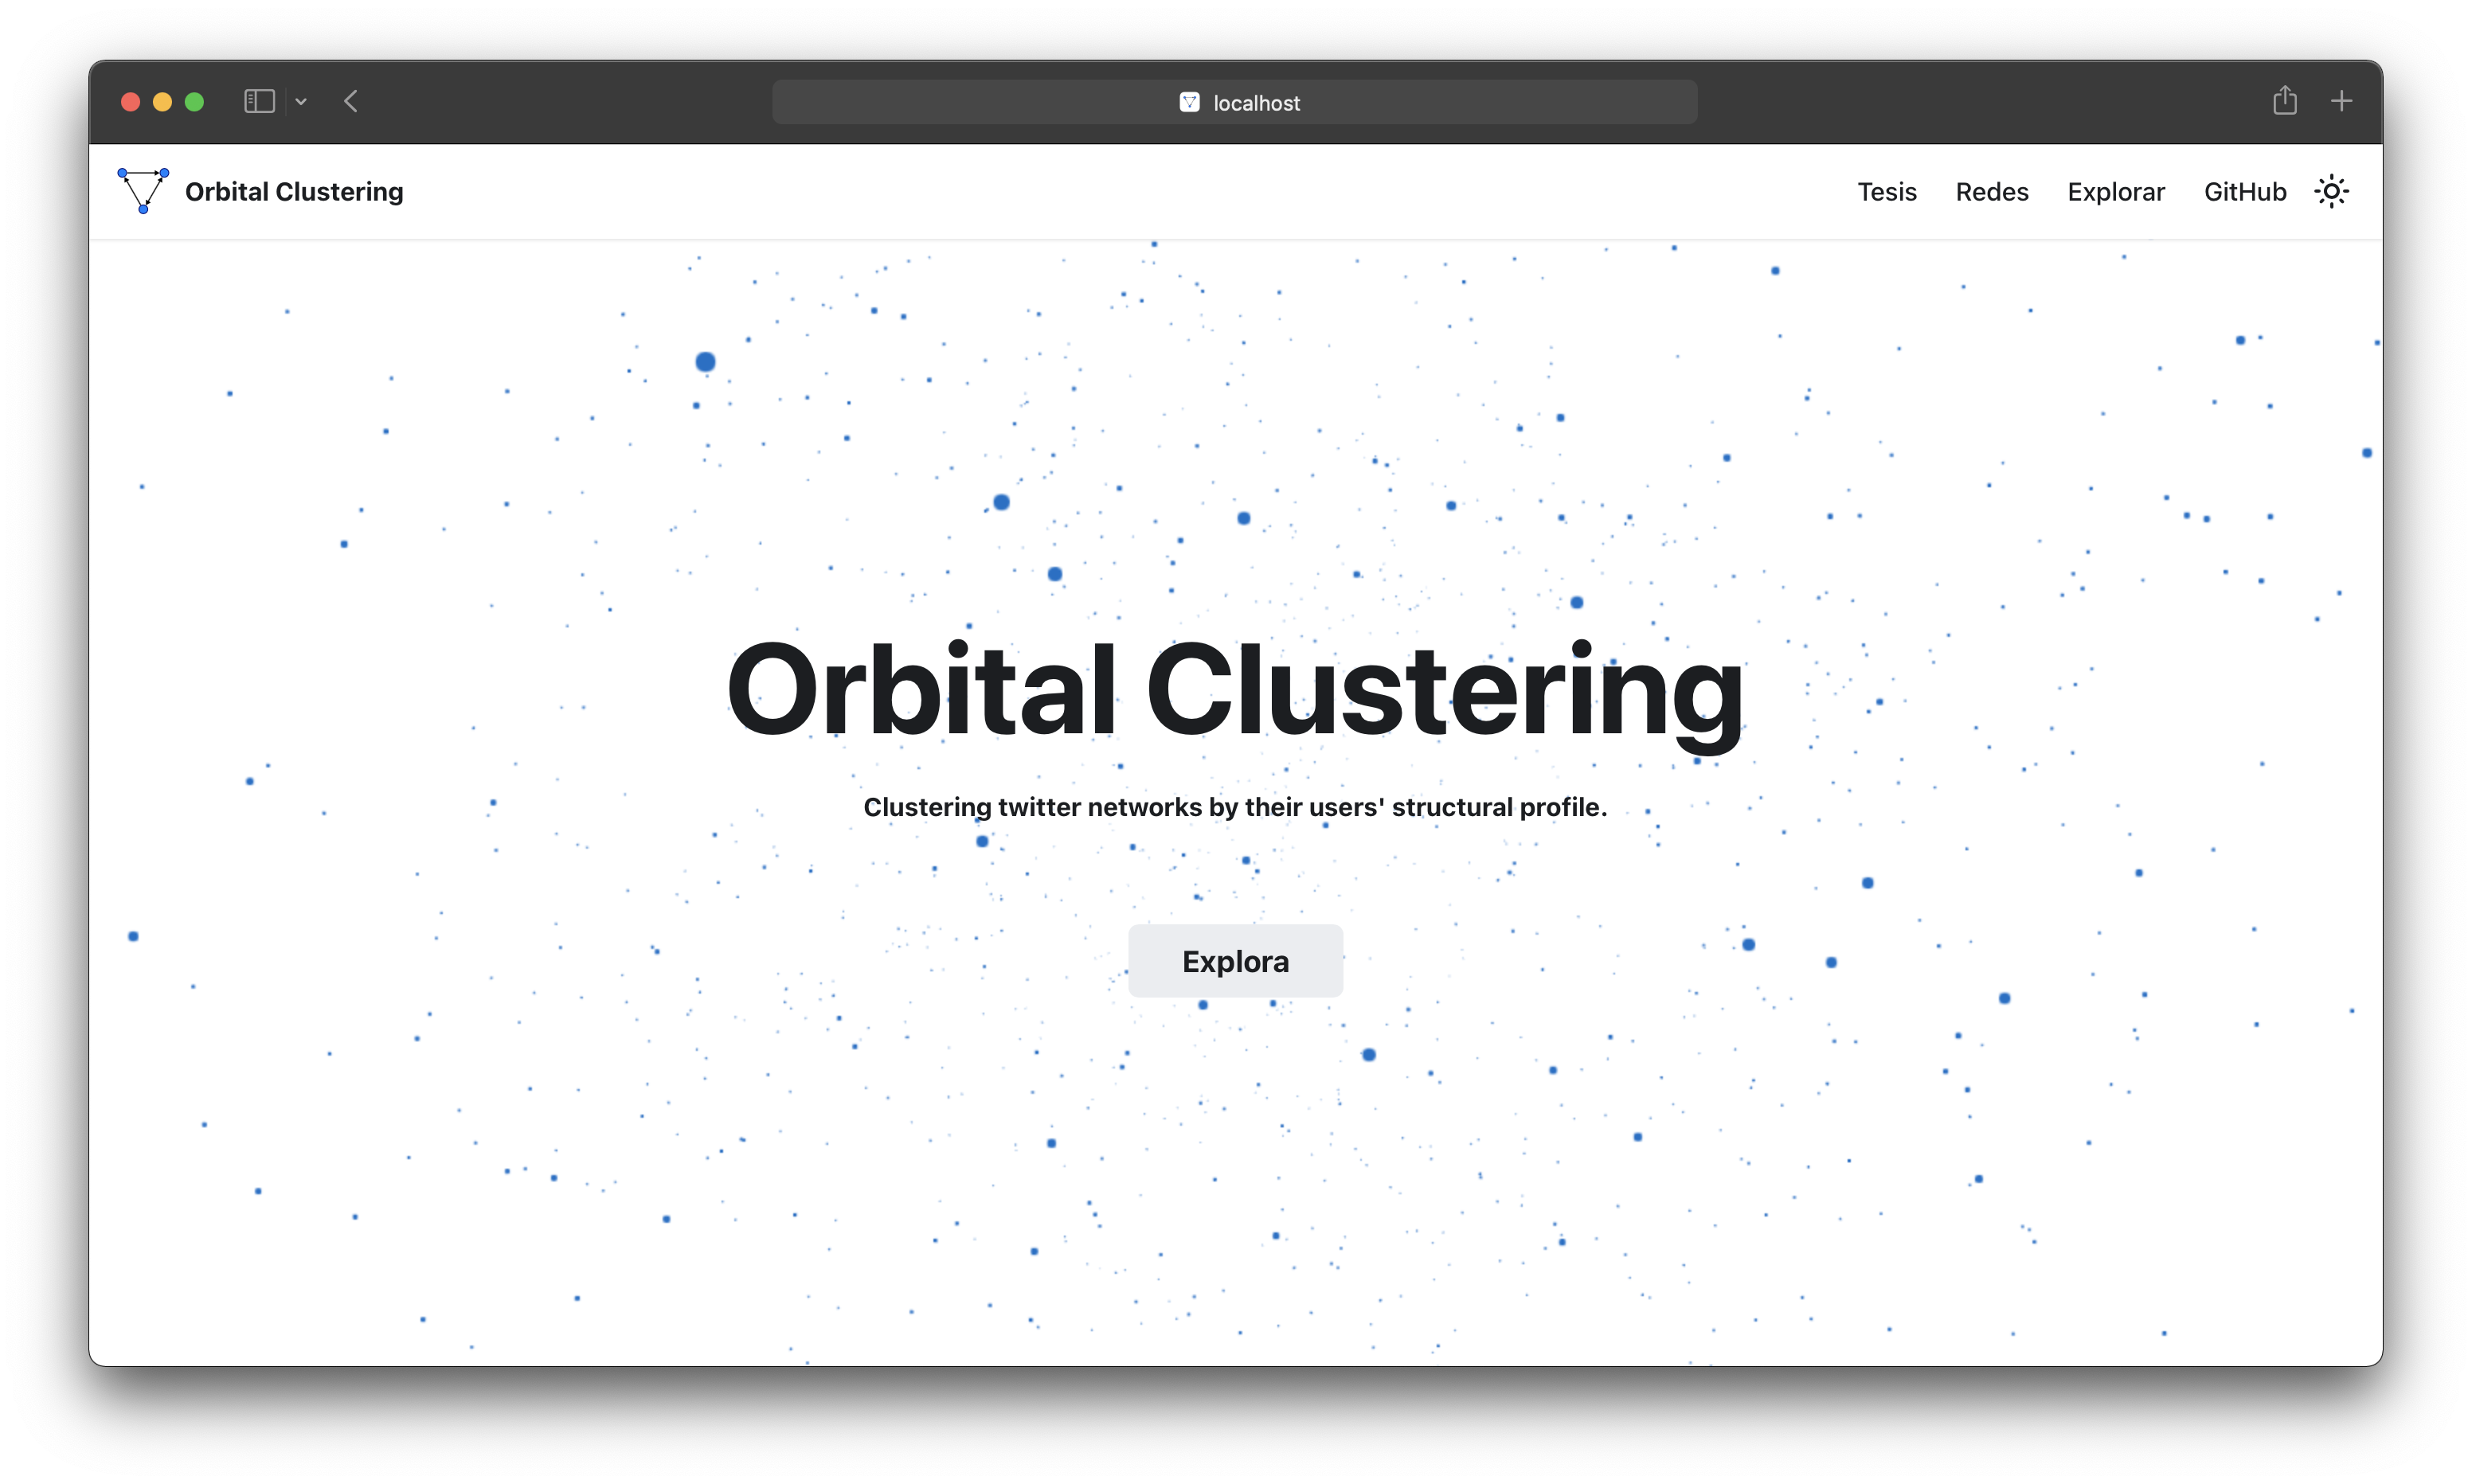
\includegraphics[width=1\textwidth]{images/web-main.png}
    \caption{Página principal de la sitio web.}
    \label{img:web-main}
\end{figure}

La herramienta web tiene distintas pestañas que permiten explorar distintos aspectos de nuestro trabajo. La primera, permite explorar con una gráfica de radar la composición por tipo de usuarios de la red seleccionada. La Fig. \ref{img:web-comp} ejemplifica la composición de una de las redes temáticas en la colección.

 \begin{figure}
   \centering
   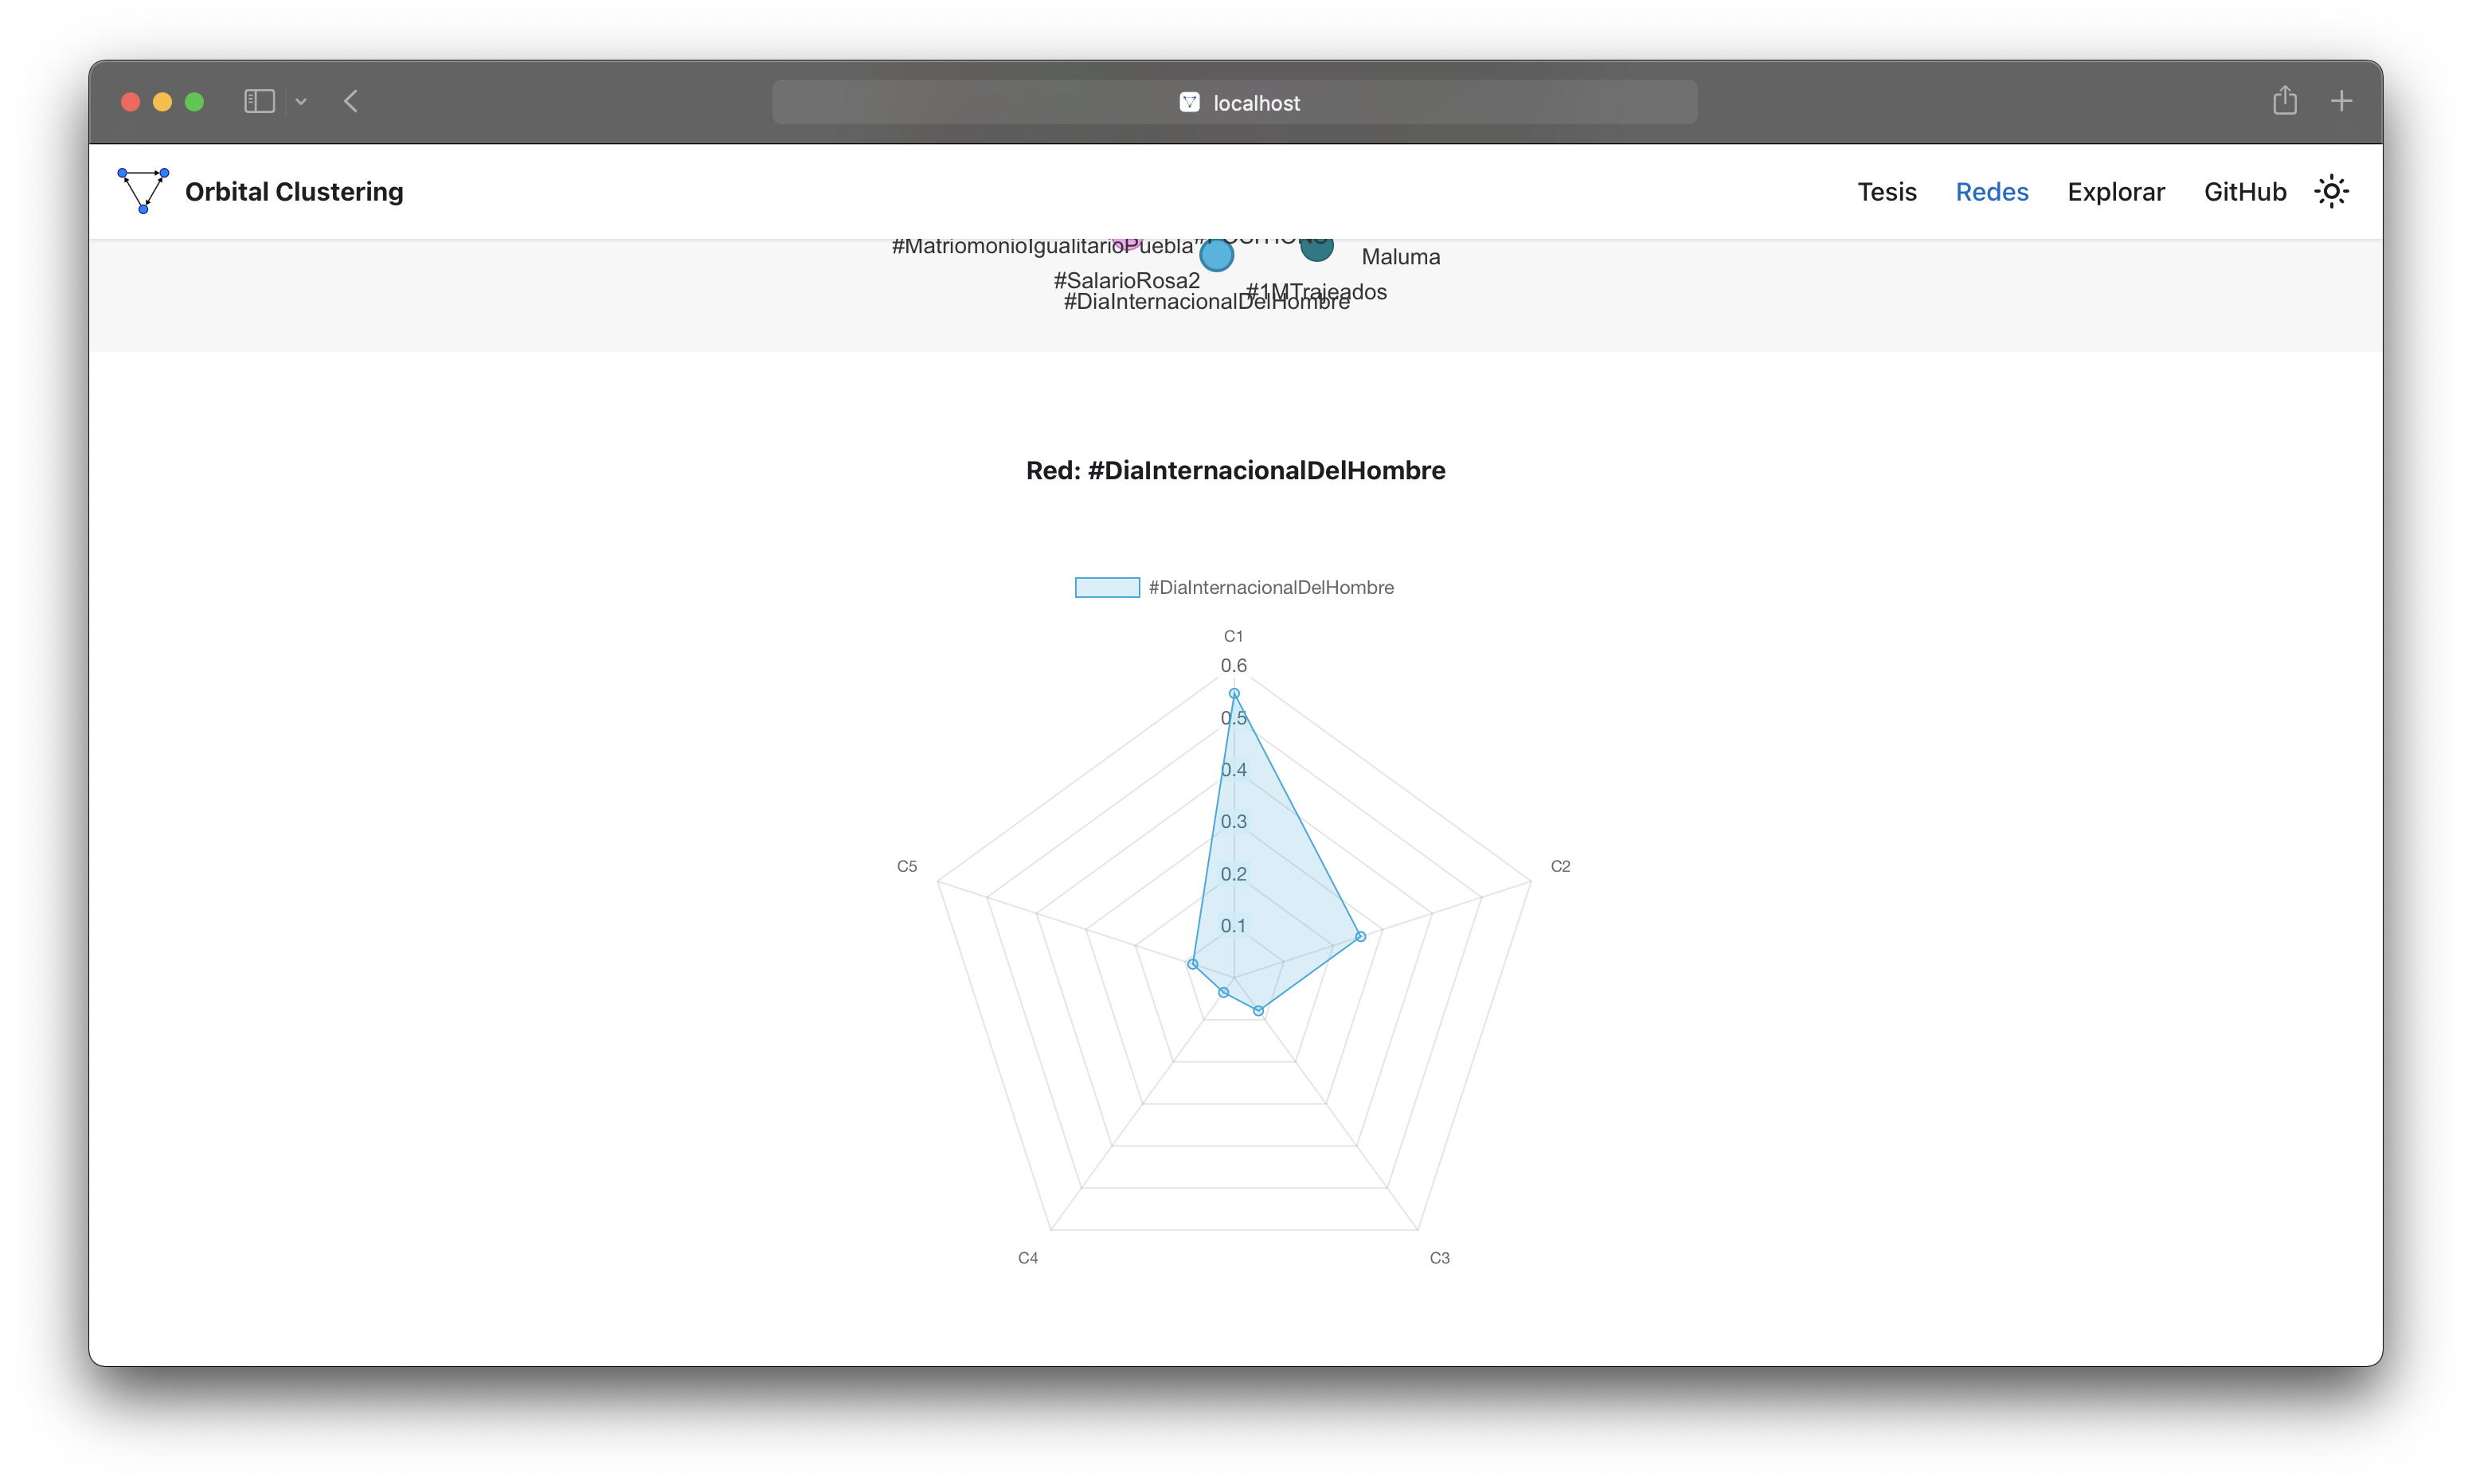
\includegraphics[width=1\textwidth]{images/web-comp.png}
    \caption{Ejemplo de la visualización de la composición de una red utilizando una gráfica de radar.}
    \label{img:web-comp}
\end{figure}

Otra de las funciones principales es la visualización de los grafos con sus respectivos nodos coloreados de acuerdo al perfil que pertenecen. La Fig. \ref{img:web-graph} nos muestra la red de \#Coco, visibilizando algunas interacciones dentro de la red.

 \begin{figure}
   \centering
   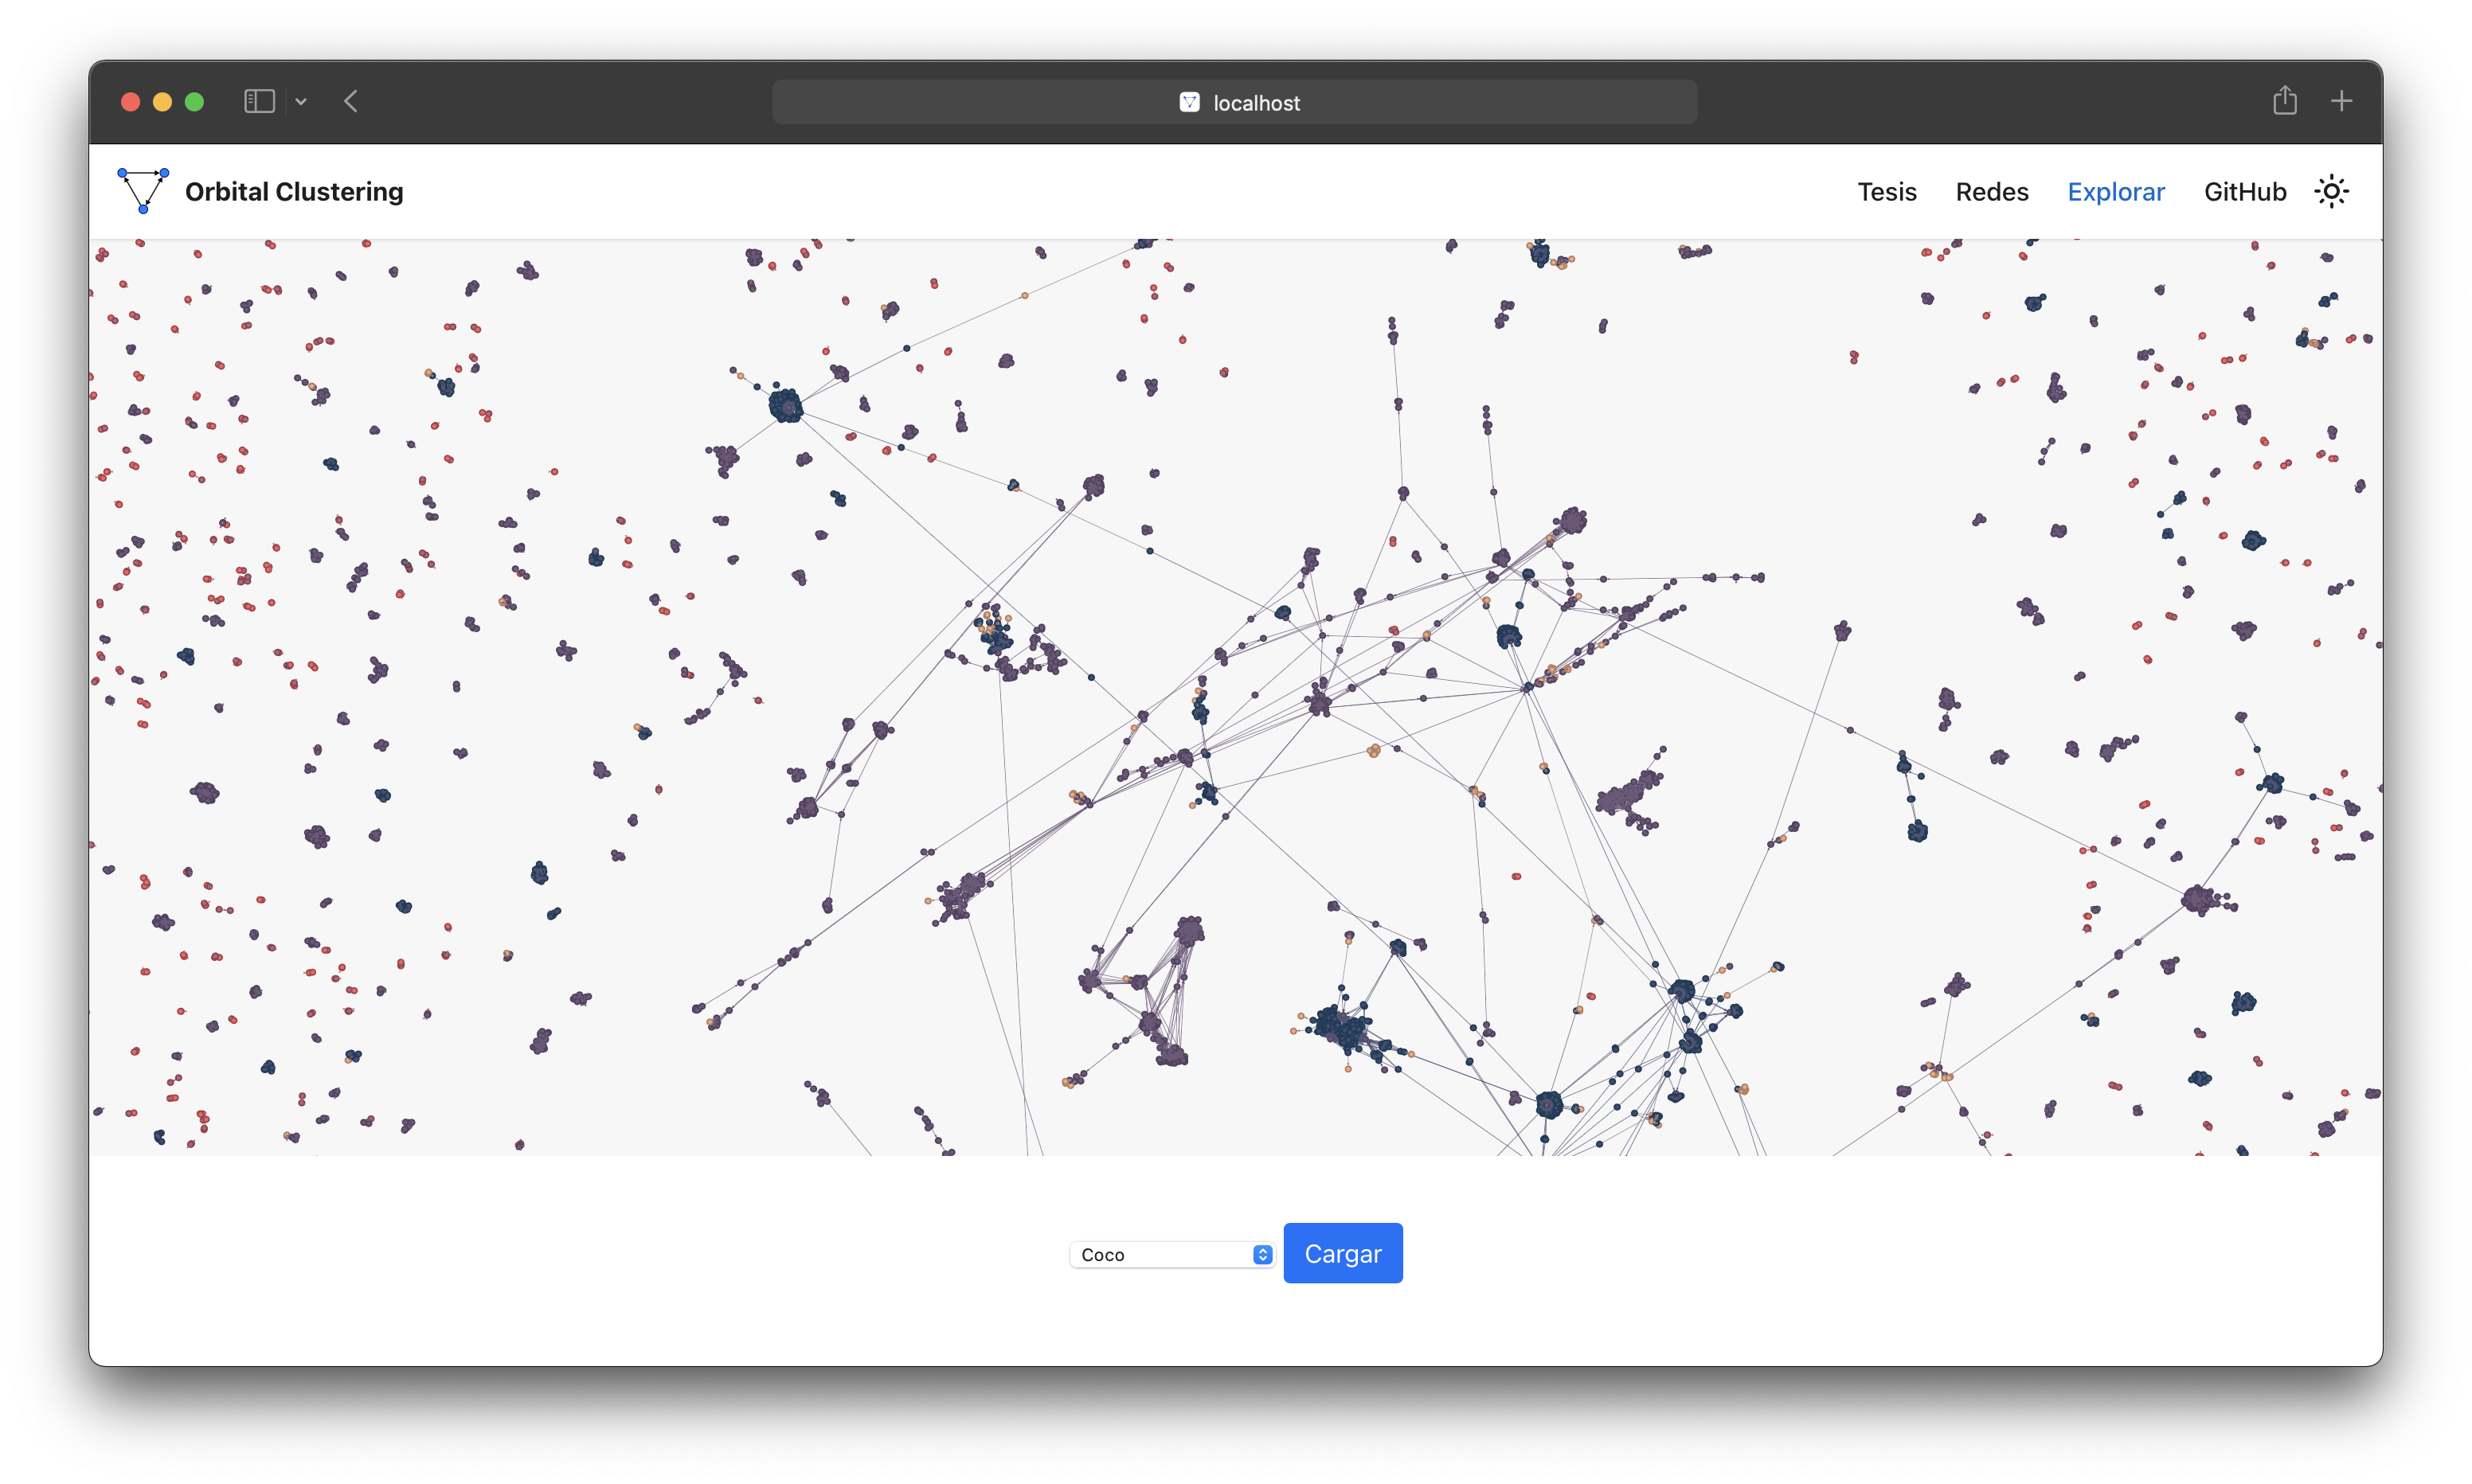
\includegraphics[width=1\textwidth]{images/web-graph.png}
    \caption{Ejemplo de la visualización de una red (\#Coco) dentro de la herramienta web.}
    \label{img:web-graph}
\end{figure}

Los grafos que se muestran a continuación (Figs. \ref{fig:net-salario} y \ref{fig:net-coco}) fueron escogidos como ejemplos por ser los más lejanos de acuerdo al agrupamiento jerárquico. En la Fig. \ref{fig:net-salario} observamos la red correspondiente al \#SalarioRosa, en la que la mayoría de las cuentas interactúan con un único usuario. Este tipo de comportamiento podría sugerir que el \textit{hashtag} (\#) nace a partir de un gran influenciador o que se trata de cuentas automatizadas que tienen el objetivo de hacer central a un usuario en la red. En contraste, la Fig. \ref{fig:net-coco} muestra una red más bien fragmentada en la que no existe una conversación central. La Tabla \ref{table:comparacionCocoSalarioRosa} presenta el contraste entre los $embeddings$ generados para ambas redes.

\begin{figure}
    \centering
    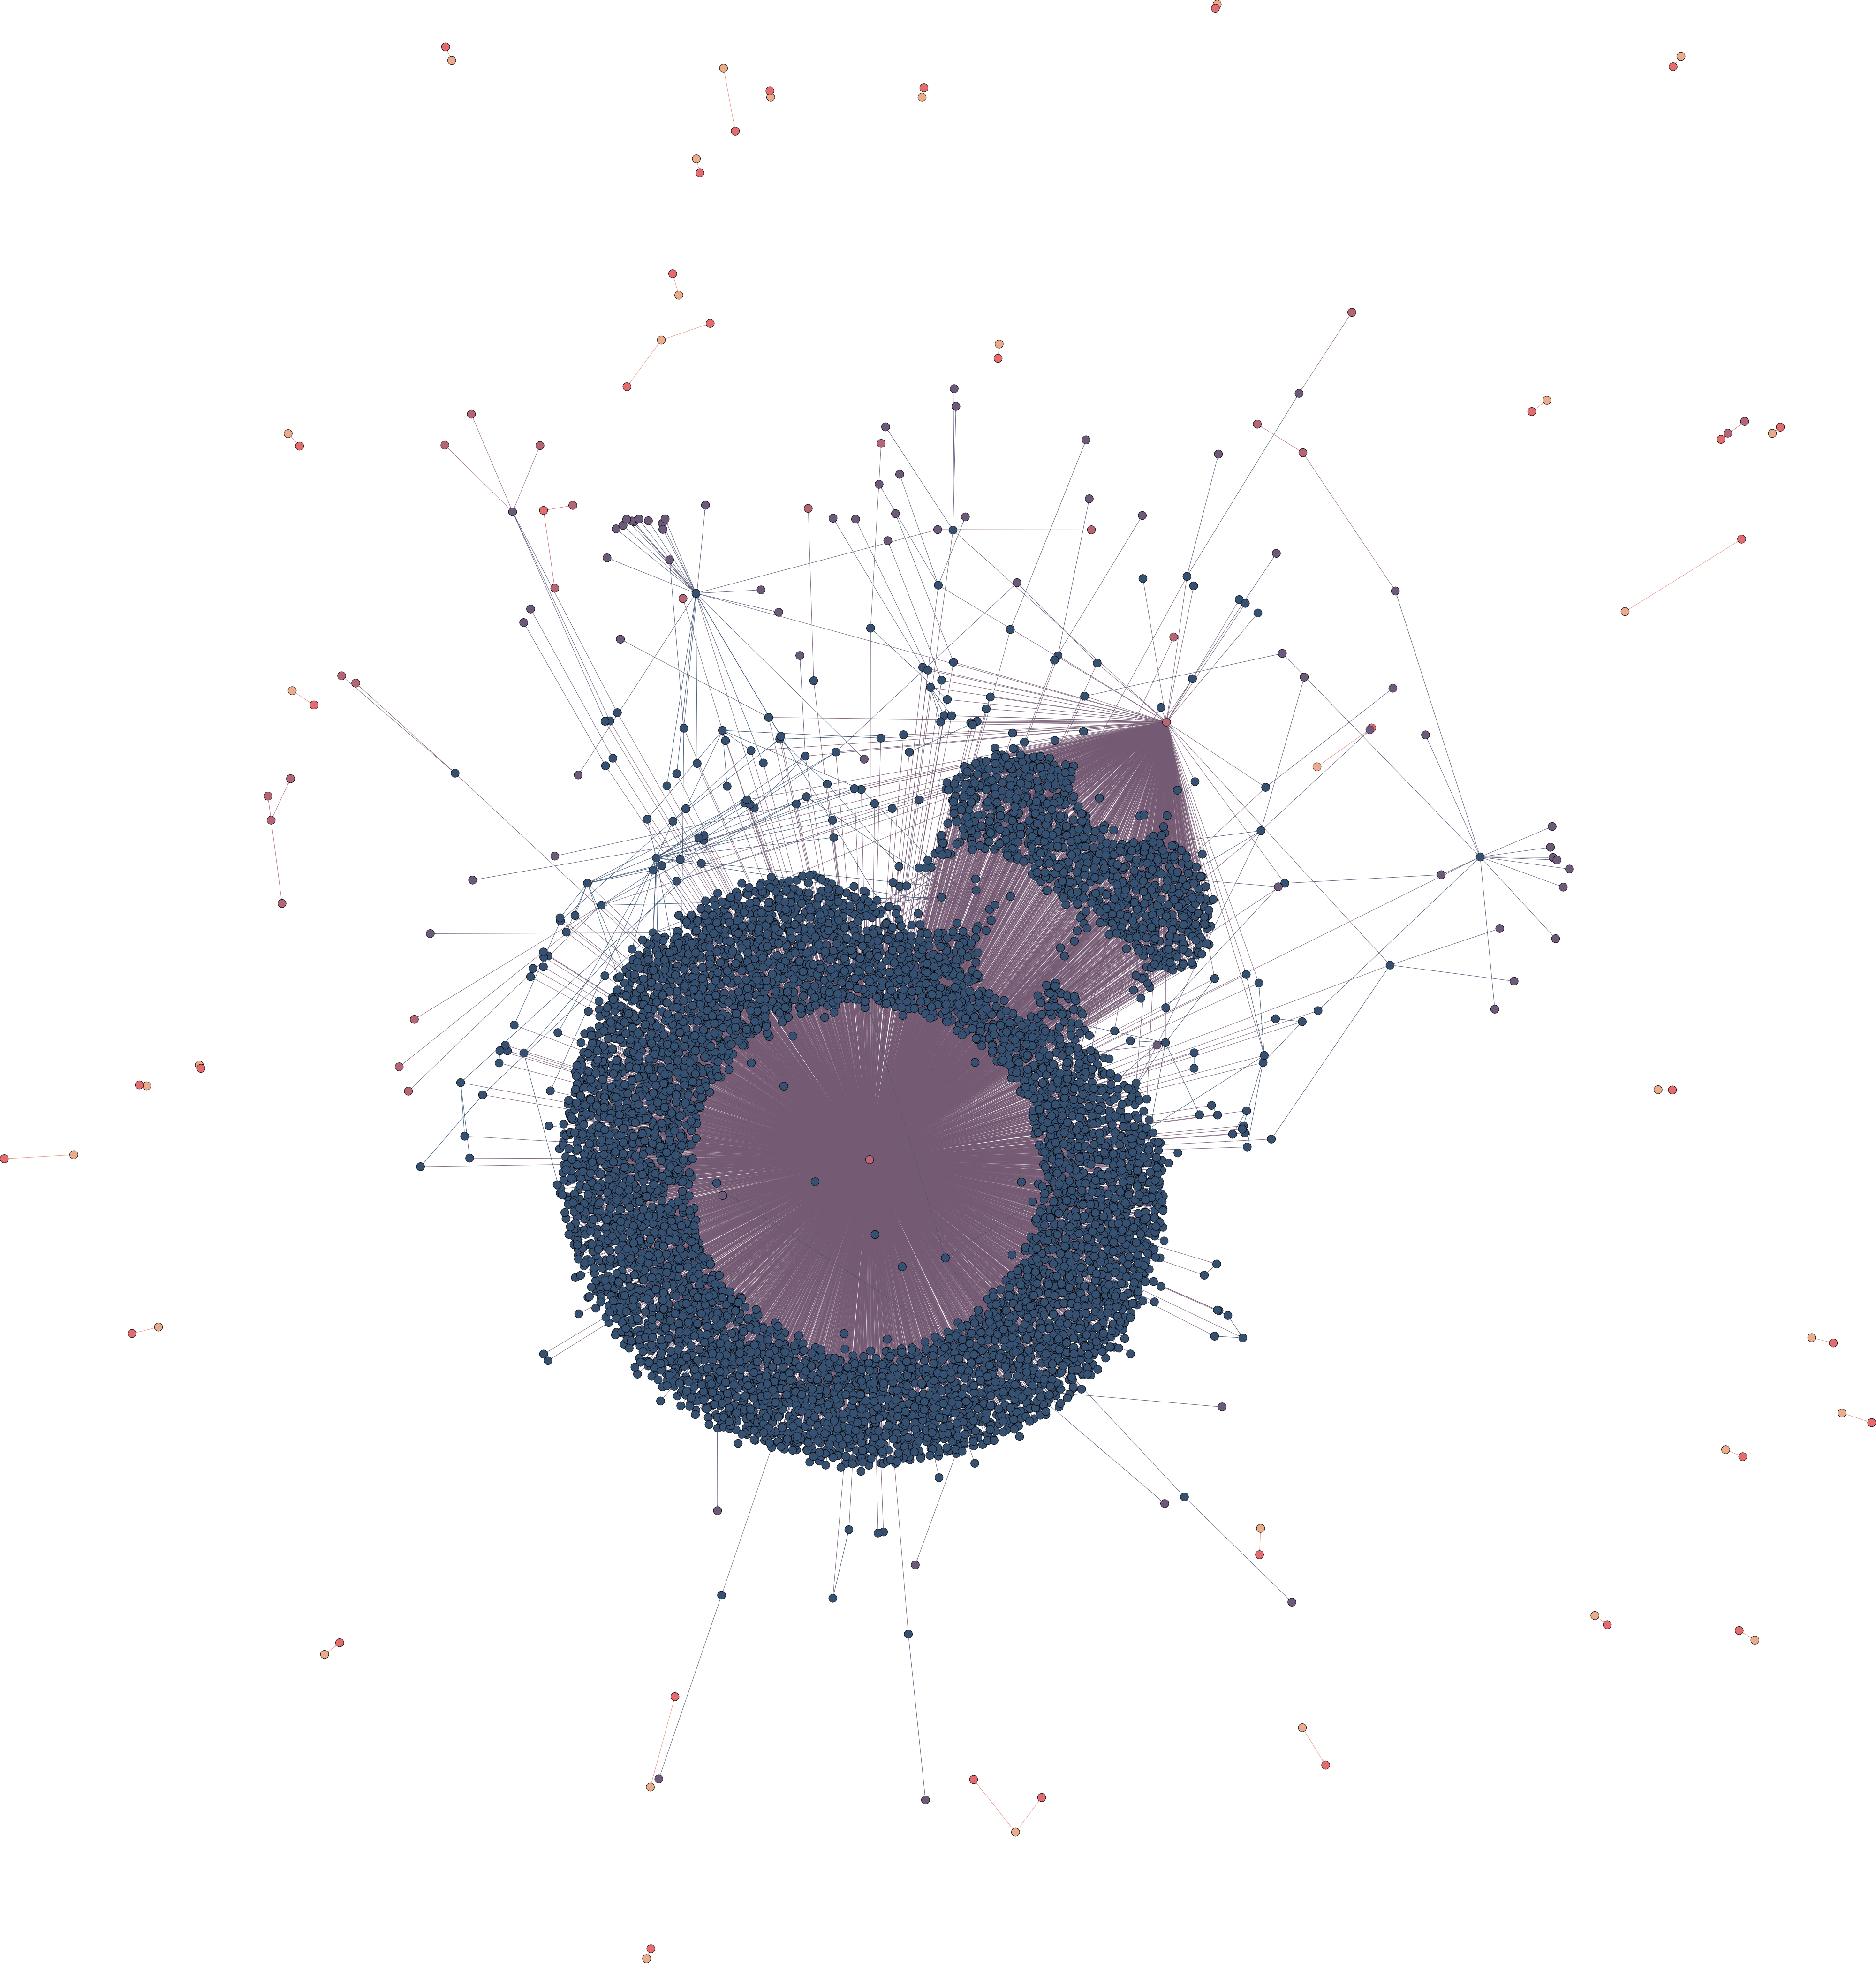
\includegraphics[width=.75\textwidth]{images/SalarioRosa.png}
    \caption{Red \#SalarioRosa coloreada respecto al grupo al que pertenece cada nodo en la red.}
    \label{fig:net-salario}
\end{figure}

\begin{figure}
    \centering
    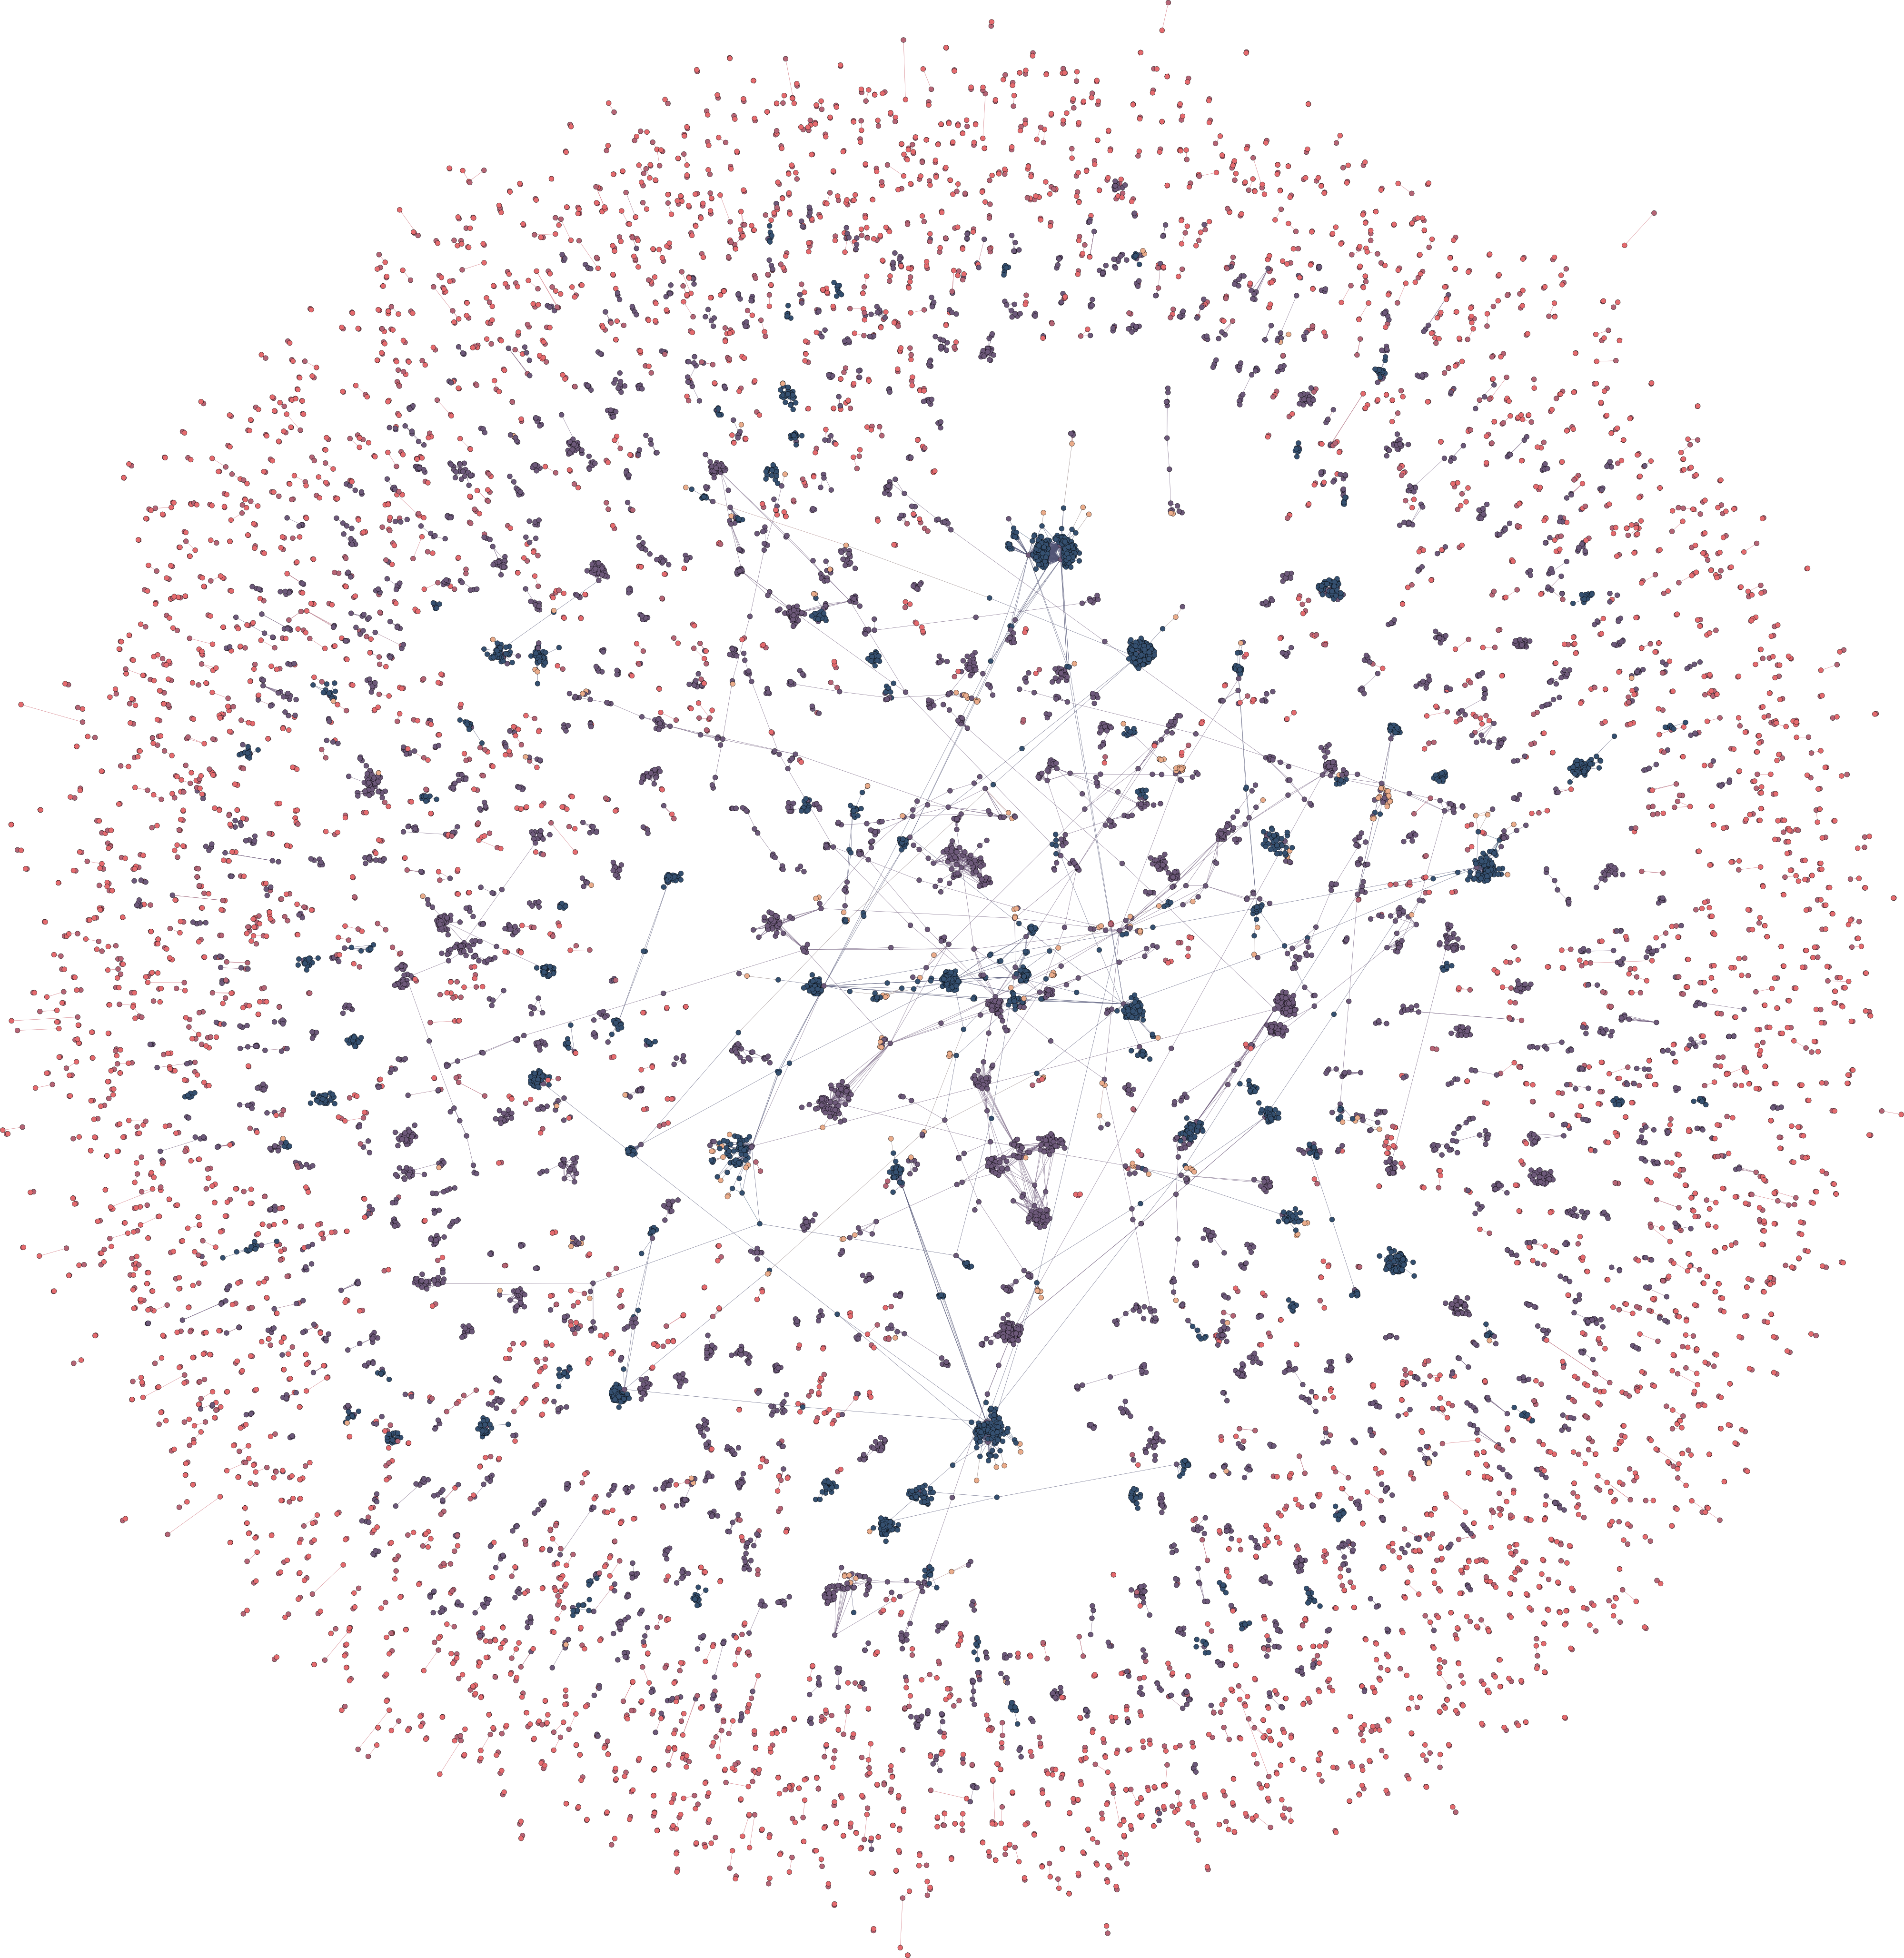
\includegraphics[width=.75\textwidth]{images/Coco.png}
    \caption{Red \#Coco coloreada respecto al grupo al que pertenece cada nodo en la red.}
    \label{fig:net-coco}
\end{figure}


\begin{table}[h]
\centering
        \csvautotabular{csv/embeddings-comp.csv}
        \newline
        \caption{Comparación de los \textit{embeddings} de las redes de \#Coco y \#SalarioRosa}
        \label{table:comparacionCocoSalarioRosa}
\end{table}


\section{Discusión}
En el conjunto de datos analizado, cuatro de los perfiles (1, 2, 4, 5) se distinguen por la presencia de una órbita dominante en el vector centroide representativo. En cambio, el grupo restante (3) tiene una distribución de órbitas más equilibrada en el vector de firmas de su centroide.

A continuación, se presenta una caracterización para cada uno de los perfiles de usuario identificados. Aunque la discusión se centra en los perfiles específicos identificados para esta colección, ejemplifica el tipo de análisis que puede derivarse de la metodología propuesta en este trabajo.   

\begin{itemize} 
    
\item \emph{Perfil 1, Reportero.} La órbita dominante es la 29, que desempeña todos los papeles de oyente en el \textit{graphlet} de un triodo. Esta órbita dominante desempeña el papel de oyente. Analizando los vecindarios con tres nodos, es infrecuente que este perfil participe en rutas con una longitud superior a uno o que responda a tweets de dos nodos diferentes, pero es habitual que el usuario responda a tweets que están siendo contestados por una o dos personas más. Así, podríamos decir que este tipo de usuario tiende a responder a tweets y usuarios que son populares. Dado que este perfil incluye todas las órbitas, podríamos decir que estos usuarios tienen más impacto en la conversación que los repetidores. \begin{figure}[htbp]
   \centering
   \includesvg[width=0.2\textwidth]{figures/G10.svg}
    \caption{Graphlet 10 y órbitas 29 y 30.}
    \label{fig:G10}
\end{figure}

\item \emph{Perfil 2, Inconformista.} La órbita dominante es la 24, que desempeña el papel de hablante en un \textit{graphlet} de 4 nodos. La particular arquitectura de este \textit{graphlet} sugiere la presencia de nodos que recogen información de diferentes fuentes y que no interactúan entre sí. El comportamiento sugiere que este usuario participa en una discusión más amplia con un punto de vista parcial. \begin{figure}[htbp]
   \centering
   \includesvg[width=0.05\textwidth]{figures/G8.svg}
    \caption{Graphlet 8 y órbitas 21 a 24.}
    \label{fig:G8}
\end{figure}

\item \emph{Perfil 3, Conversador.} En este perfil aparecen todas las órbitas incluyendo aquellas dominantes de los otros cuatro perfiles. Las órbitas dominantes en este perfil son la 29, 7, 17, 21 y 31. Las mayoría de las órbitas son oyentes, pero la órbita 31 desempeña todos los papeles de pozo en un \textit{graphlet} de 4 nodos. La variedad de roles que puede adoptar este grupo de usuarios, se ve reflejada en la composición equilibrada de los vectores de firmas asociados, lo que sugiere que este perfil permite el flujo de información hacia y desde los otros perfiles predominantes.

\item \emph{Perfil 4, Difusor.} La órbita dominante es la 1, que desempeña el papel de un pozo en el \textit{graphlet} compuesto por un solo arco. Las órbitas 2, 6 y 11 (todas ellas órbitas fuente) nunca aparecen en los vectores de firmas de estos usuarios. Analizando los vecindarios con tres nodos, las pocas veces que este perfil desempeña el papel de oyente, también lo hace de audiencia. Dada la alta frecuencia de la órbita dominante, es razonable suponer que estos usuarios producen información que motiva a los lectores a responder. 
\begin{figure}[htbp]
   \centering
   \includesvg[width=0.25\textwidth]{figures/Or-1.svg}
    \caption{Graphlet 0 y órbita 1.}
    \label{fig:0-1}
\end{figure}

\item \emph{Perfil 5, Repetidor.} La órbita dominante es la 0, que desempeña el papel de oyente en un \textit{graphlet} de arco, pero no tiene el papel de audiencia. La mayoría de las otras órbitas no aparecen asociadas a este tipo de usuario. En particular, si observamos todos los vecindarios con dos y tres nodos, este perfil nunca es retuiteado o mencionado por otro usuario. Además, observamos que el usuario no participa en \textit{graphlets} de tamaño cuatro y, por tanto, tampoco en vecindarios más grandes. A partir de los roles recurrentes encontrados en esta órbita, podríamos decir que estos usuarios tienden a repetir los mensajes en la mayoría de sus interacciones sin impactar significativamente en la conversación. \begin{figure}[htbp]
   \centering
   \includesvg[width=0.25\textwidth]{figures/Or-0.svg}
    \caption{Graphlet 0 y órbita 0.}
    \label{fig:0-0}
\end{figure}


\end{itemize}

Las órbitas 30, 63, 85, 91, 105, 118 y 125 son hablantes con un grado de salida igual a 3, que aparecen con muy poca frecuencia en las firmas de los perfiles identificados. Es de esperar que estas órbitas aparezcan en usuarios reconocidos como \textit{Influencers} de la red. La presencia de la órbita 29 en el perfil de Reportero sugiere que la órbita 30 aparece varias veces en una red. Curiosamente, la órbita 30 aparece de forma distribuida, sin ser la órbita principal en los perfiles Difusor, Conversador o Inconformista.

En cuanto a la agrupación de las redes, la metodología propuesta permite ordenar la colección y definir grupos interpretables que proporcionan una visión de la dinámica originada por los diferentes temas. Los grupos no responden a una diferenciación temática, lo que refuerza la idea de que los procesos de difusión en Twitter no dependen sólo del contenido. No obstante, el análisis revela diferencias entre las redes sugiriendo una clara variación en cuanto a roles que emergen entre los usuarios y el efecto que esto tiene en la circulación de ideas a través de Twitter. 

En el grupo de las redes que muestran una alta inequidad en las opiniones propagadas (redes más a la izquierda en la Fig. \ref{fig:composition}), con unas pocas voces autorizadas (difusores) de las que se hacen eco otros perfiles (reporteros), encontramos algunas iniciativas gubernamentales (\#SalarioRosa, \#OfrendaEdoMex, \#TarjetaRosa). Podría darse el caso de que algunos tweets sean lanzados y manejados estratégicamente para aumentar su importancia. En el otro lado del espectro (instancias más a la derecha en la Fig. \ref{fig:composition}), encontramos redes temáticas relacionadas con películas y temas generales (Coco, Karol, \#FelizMiercoles) que abarcan un intercambio de información más distribuido, lo que sugiere un tema con un mayor nivel de participación y menos voces predominantes sobre el tema. 

   % INCLUDE: Experimentos y resultados

\chapter{Conclusiones}
\label{sec:conclusion}

Con el uso de modelos basados en redes en diferentes disciplinas del conocimiento, el agrupamiento en conjuntos de redes se vuelve una tarea muy importante. Sin embargo, no todos los métodos existentes proporcionan resultados que puedan traducirse fácilmente a nuevas interpretaciones de los datos. 

En este trabajo se presenta una alternativa para agrupar redes sociales. El método propuesto tiene dos etapas principales: detectar el perfil de usuarios con base en su firma orbital en graphlets, y agrupar las redes de acuerdo a la caracterización de usuarios que las conforman.  

La metodología presentada utiliza algoritmos computacionales ampliamente conocidos con implementaciones eficientes que permiten el desarrollo de cada paso propuesto. De este modo, nuestro enfoque aprovecha la utilidad de los graphlets y de sus órbitas asociadas para capturar información sobre la estructura de una red y llevar a cabo tareas de agrupamiento.

%Nuestro enfoque es interpretable y capaz de captar la estructura de la red mediante el uso de graphlets.
%con un método que provee información sobre la similitud entre redes basado en perfiles de usuario y sus roles estructurales a través de representaciones vectoriales (embeddings)
 
Mostramos la utilidad de la metodología propuesta a través de una aplicación real con redes temáticas de Twitter. Encontramos que los perfiles establecidos en el primer paso del método nos dan información útil sobre las estructuras de la red y las dinámicas sociales dentro de ellas. Esta descripción de perfiles puede considerarse una extensión de trabajo propuesto en sociología que sólo consideraba triadas de nodos. El método también reconoce que un usuario puede tener varios roles dentro de la discusión sobre un cierto tema en Twitter. 

% Pasar a conclusiones 
Consideramos que nuestro enfoque tiene al menos dos ventajas. En primer lugar, proporciona un método para agrupar redes temáticas de Twitter de forma explicable, capturando las diferencias entre ellas que van más allá de las métricas generales de la red. En segundo lugar, produce una caracterización de los usuarios de la red que puede ayudar a comprender la estructura, las relaciones y los patrones latentes creados por la compleja dinámica de Twitter. 

Entre las líneas de trabajo futuro que se proponen, está la posibilidad de explorar la generalidad de los perfiles de usuario detectados. Además, queda por hacer un análisis más detallado de estos perfiles con un punto de vista interdisciplinario. Es decir, la discusión aún puede ser extendida con herramientas y metodologías de otras áreas afines, por ejemplo de las ciencias sociales.   % INCLUDE: Conclusiones

% --------------------------
% Back matter
% --------------------------
%

%\cleardoublepage

%\listoffigures
%\cleardoublepage

%\listoftables
%\cleardoublepage

%\lstlistoflistings
%\cleardoublepage

\appendix\cleardoublepage

\chapter{Apéndice}
\label{sec:appendix}

\section{Capítulo 1}
\label{sec:appendix:c2}

\subsubsection{Homofilia}

En sociología se denomina homofilia (del griego «amor a los iguales») a la tendencia de las personas por la atracción a sus homónimos. Esta atracción puede ser respecto a distintos atributos como edad, género, creencias, educación, estrato social, etc.

\subsubsection{Centralidad de Intermediación}

La distancia de intermediación o \textit{Betweenes Centrality} es una medida de centralidad basada en geodésicas o caminos más cortos \cite{wikipedia_betweenness_nodate}.

Formalmente esta definida como:

$$g(v)=\sum _{{s\neq v\neq t}}{\frac  {\sigma _{{st}}(v)}{\sigma _{{st}}}}$$

donde $\sigma_{st}$ es el número total de caminos mas cortos desde el nodo $s$ al nodo $t$ y $\sigma_{st}(v)$ es el número total de esos caminos que pasan a través de $v$ (dónde $v$ no es el nodo final de un camino).

\section{Capítulo 2}
\label{sec:appendix:c2}

\subsubsection{Función Biyectiva}

Una función es biyectiva es aquella que es a la vez inyectiva y suprayectiva. Es decir, una función entre los elementos de dos conjuntos, donde cada elemento de un conjunto se empareja con exactamente un elemento del otro conjunto, y cada elemento del otro conjunto se empareja con exactamente un elemento del primer conjunto.

Formalmente, dada una función $f$

$ {\begin{array}{rccl}f:&X&\longrightarrow &Y\\&x&\longmapsto &y=f(x)\end{array}} $

Es biyectiva si para todo $y$ de $Y$ existe un único $x$ de $X$ al que la función evaluada en $x$ es igual a $y$

$ \forall y\in Y\;:\quad \exists !\ x\in X\;/\quad f(x)=y $

\section{Capítulo 5}
\label{sec:appendix:c3}

\subsubsection{Línea base}
\label{sec:appendix:baseline}

Utilizando el árbol de decisión de \textit{Himelboim et. al} \cite{himelboim_classifying_2017} se clasificó el conjunto de datos de redes temáticas de Twitter para establecer una línea base. En este caso el agrupamiento no es óptimo ya que la mayoría de las redes quedan en un solo grupo.

\begin{table}[h]
\begin{center}
    \csvautotabular{csv/baseline1.csv}
    \caption{Resultado del agrupamiento realizado utilizando el árbol de decisión de \cite{himelboim_classifying_2017} para el conjunto de redes temáticas.}
\end{center}
\end{table}

\begin{table}[h]
\begin{center}
    \csvautotabular{csv/baseline2.csv}
    \caption{Resultado del agrupamiento realizado utilizando el árbol de decisión de \cite{himelboim_classifying_2017} para el conjunto de redes temáticas.}
\end{center}
\end{table}       % INCLUDE: appendix

{%
\setstretch{1.1}
\renewcommand{\bibfont}{\normalfont\small}
\setlength{\biblabelsep}{0pt}
\setlength{\bibitemsep}{0.5\baselineskip plus 0.5\baselineskip}
\printbibliography[]
%\printbibliography[nottype=online]
%\newrefcontext[labelprefix={@}]
%\printbibliography[heading=subbibliography,title={Webpages},type=online]

}

\newpage
\mbox{}

% **************************************************
% End of Document CONTENT
% **************************************************
\end{document}
